\documentclass[phd]{ucbthesis}

\usepackage{url}
\usepackage{algorithmic}
\usepackage{algorithm}
\usepackage{listings}
\usepackage{balance}
\usepackage{graphicx}
\usepackage{hyperref}
\usepackage{amsthm}
\usepackage{multirow}
\usepackage{xfrac}

\newtheorem{defn}{Definition}
\newtheorem{lemma}{Lemma}

% \usepackage{draftwatermark}
% \SetWatermarkText{DRAFT}
% \SetWatermarkScale{5}
% "define" Scala
\lstdefinelanguage{scala}{morekeywords={class,object,trait,extends,with,new,if,while,for,def,val,var,this},
otherkeywords={->,=>},
sensitive=true,
morecomment=[l]{//},
morecomment=[s]{/*}{*/},
morestring=[b]"}
% Default settings for code listings
\lstset{frame=tb,language=scala,aboveskip=3mm,belowskip=3mm,showstringspaces=false,columns=flexible,basicstyle={\small\ttfamily}}
\usepackage{amsmath}

\begin{document}

\frontmatter

\title{Scalable Systems and Algorithms for Genomic Variant Analysis}
\author{Frank Austin Nothaft}
\degreesemester{Fall}
\degreeyear{2017}
\degree{Doctor of Philosophy}
\chair{Professor Anthony Joseph}
\cochair{Professor David Patterson}
\othermembers{Professor Haiyan Huang}
\numberofmembers{3}
\field{Computer Science}
\campus{Berkeley}

\maketitle

\approvalpage
\copyrightpage

\begin{abstract}
  With the cost of sequencing a human genome dropping below \$1,000,
  population-scale sequencing has become feasible. With projects that sequence
  more than 10,000 genomes becoming commonplace, there is a strong need for
  genome analysis tools that can scale across distributed computing
  resources while providing reduced analysis cost. Simultaneously, these tools
  must provide programming interfaces and deployment models that are easily
  usable by biologists.

  In this dissertation, we describe the \textsc{ADAM} system for processing
  large genomic datasets using distributed computing. \textsc{ADAM} provides
  a decouped stack-based architecture that can accomodiate many data formats,
  deployment models, and data access patterns. Additionally, \textsc{ADAM}
  defines schemas that describe common genomic datatypes. \textsc{ADAM}'s
  schemas and programming models enable the easy integration of disparate
  genomic datatypes and datasets into a single analysis.

  To validate the \textsc{ADAM} architecture, we implemented an end-to-end
  variant calling pipeline using \textsc{ADAM}'s APIs. To perform parallel
  alignment, we developed the \textsc{Cannoli} tool, which uses \textsc{ADAM}'s
  APIs to automatically parallelize single node aligners. We then
  implemented \textsc{GATK}-style alignment refinement as part of \textsc{ADAM}.
  Finally, we implemented a biallelic genotyping model, and novel reassembly
  algorithms in the \textsc{Avocado} variant caller. This pipeline provides
  state-of-the-art SNV calling accuracy, along with high~(97\%) INDEL calling
  accuracy. To further validate this pipeline, we reanalyzed 270 samples from
  the Simons Genome Diversity Dataset.
\end{abstract}

\tableofcontents

\mainmatter

\part{Introduction and Principles}

\chapter{Introduction}
\label{chap:introduction}

The rapid decrease in sequencing cost has made large scale sequencing
tractible. The dramatic improvement in sequencing cost since the Human
Genome Project has enabled a human whole genome sequence~(WGS) to be
generated for under \$1,000 in wetlab costs~\cite{nhgri}. This trend
will continue for the forseeable future, as sequencing vendors like
Illumina unveil new sequencers such as the NovaSeq that provide even
higher throughput while also decreasing cost, and as radically new
sequencing technologies like Oxford Nanopore come online~\cite{jain17}.
The reduced cost of sequencing enables the use of genome sequencing in
population health research projects and clinical practice. As a result,
the total volume of sequencing data produced is expected to exceed that
of YouTube by 2021~\cite{stephens15}.

The massive scale of the sequencing data that is being acquired enables
novel insight into biological phenomena. The Exome Aggregation
project~(ExAC,~\cite{lek16})--now gnomAD--provides an especially powerful
demonstration: by sequencing more than 60,000 exomes, we have been able
to better understand the impact of genomic variation on prion
disease~\cite{minikel16} and cardiovascular disease~\cite{walsh16}, and to
better characterize the effect of structural variation~\cite{ruderfer16}.
However, this scale of data solves biological problems at the cost of techincal
and logistical problems. Data storage and transfer has become a serious problem,
and the focus of many researchers~\cite{fritz11, kozanitis11} and standards
organizations~\cite{paten15}. Not only is the volume of data large, but
expensive processing is needed to analyze the data. Due to historical design
decisions, much of this processing is currently restricted to single node
architectures that assume POSIX storage APIs. As a result, it can take
upwards of 100 hours to analyze the raw read data from a single genome.

We believe that distributed computing architectures are a good match for
genomic data analysis. Horizontally scalable storage architectures can
simultaneously provide increased data storage capacities, data access
throughput, and reduced storage cost. Because most genomic analyses are centered
on analyzing the genomic data at disparate genomic loci without coordination
between loci, most genomic analysis tasks can be executed in parallel. Even more
importantly, these analysis patterns cleanly map onto quasi-relational primitives
that are powerful and can be executed in parallel. Finally, by building upon
widely used open-source distributed processing architectures like \textsc{Apache
Spark}~\cite{zaharia12} and \textsc{Hadoop}~\cite{hadoop}, genomics can benefit
from the engineering contributions that advance these large open source projects.

In this thesis, we introduce \textsc{ADAM}, an application programming
interface~(API) for processing genomic data using Apache Spark. \textsc{ADAM}
is based around a novel stack-oriented architecture that uses schemas to define
the narrow waist in the stack. On top of the schemas, we provide high-level
APIs that allow computational biologists and bioinformaticians to manipulate
collections of genomic data in a parallel fashion. The high level APIs extend
\textsc{Apache Spark}'s Resilient Distributed Dataset~(RDD, see Zahaira et
al.~\cite{zaharia12}) abstraction with genomics-specific functionality, and
eliminates the low level ``walker'' pattern~\cite{mckenna10} that is common in
genomics. At lower levels in the stack, we provide efficient implementations
of the common genomics query models. By having clearly defined APIs between
each level of the stack, we are able to exchange layers to optimize query
performance for a given query, input data type, or cluster/cloud configuration.

Our work on \textsc{ADAM} has resulted in the broad ecosystem of projects
depicted in Figure~\ref{fig:bdg}. We refer to the tools built on \textsc{ADAM}
as the ``Big Data Genomics''~(BDG) project. In this dissertation, we will limit
our focus to \textsc{ADAM}'s architecture and APIs, and the tools and algorithms
that form the core components of the BDG variant calling pipeline:

\begin{itemize}
\item \textsc{Cannoli}, which parallelizes single node genomic data processing
  tools. \textsc{Cannoli} is used in our pipeline for alignment.
\item The \textsc{ADAM} read transformations, which correct for errors in the
  aligned reads.
\item \textsc{Avocado}, a fully parallelized variant caller.
\end{itemize}

This pipeline is able to call variants on a high coverage ($60\times$) whole
genome in under one hour when running on commodity cloud computing resources.
This represents a dramatic improvement in performance over the widely used
Genome Analysis Toolkit~(GATK, see DePristo et al.~\cite{depristo11}), which
needed over 100 hours to call variants on the same sample. These tools
demonstrate how \textsc{ADAM}'s APIs enable bioinformatics analyses to be
written at a high level, while also allowing for the reuse of code from legacy
bioinformatics tools.

\begin{figure}[h]
  \begin{center}
    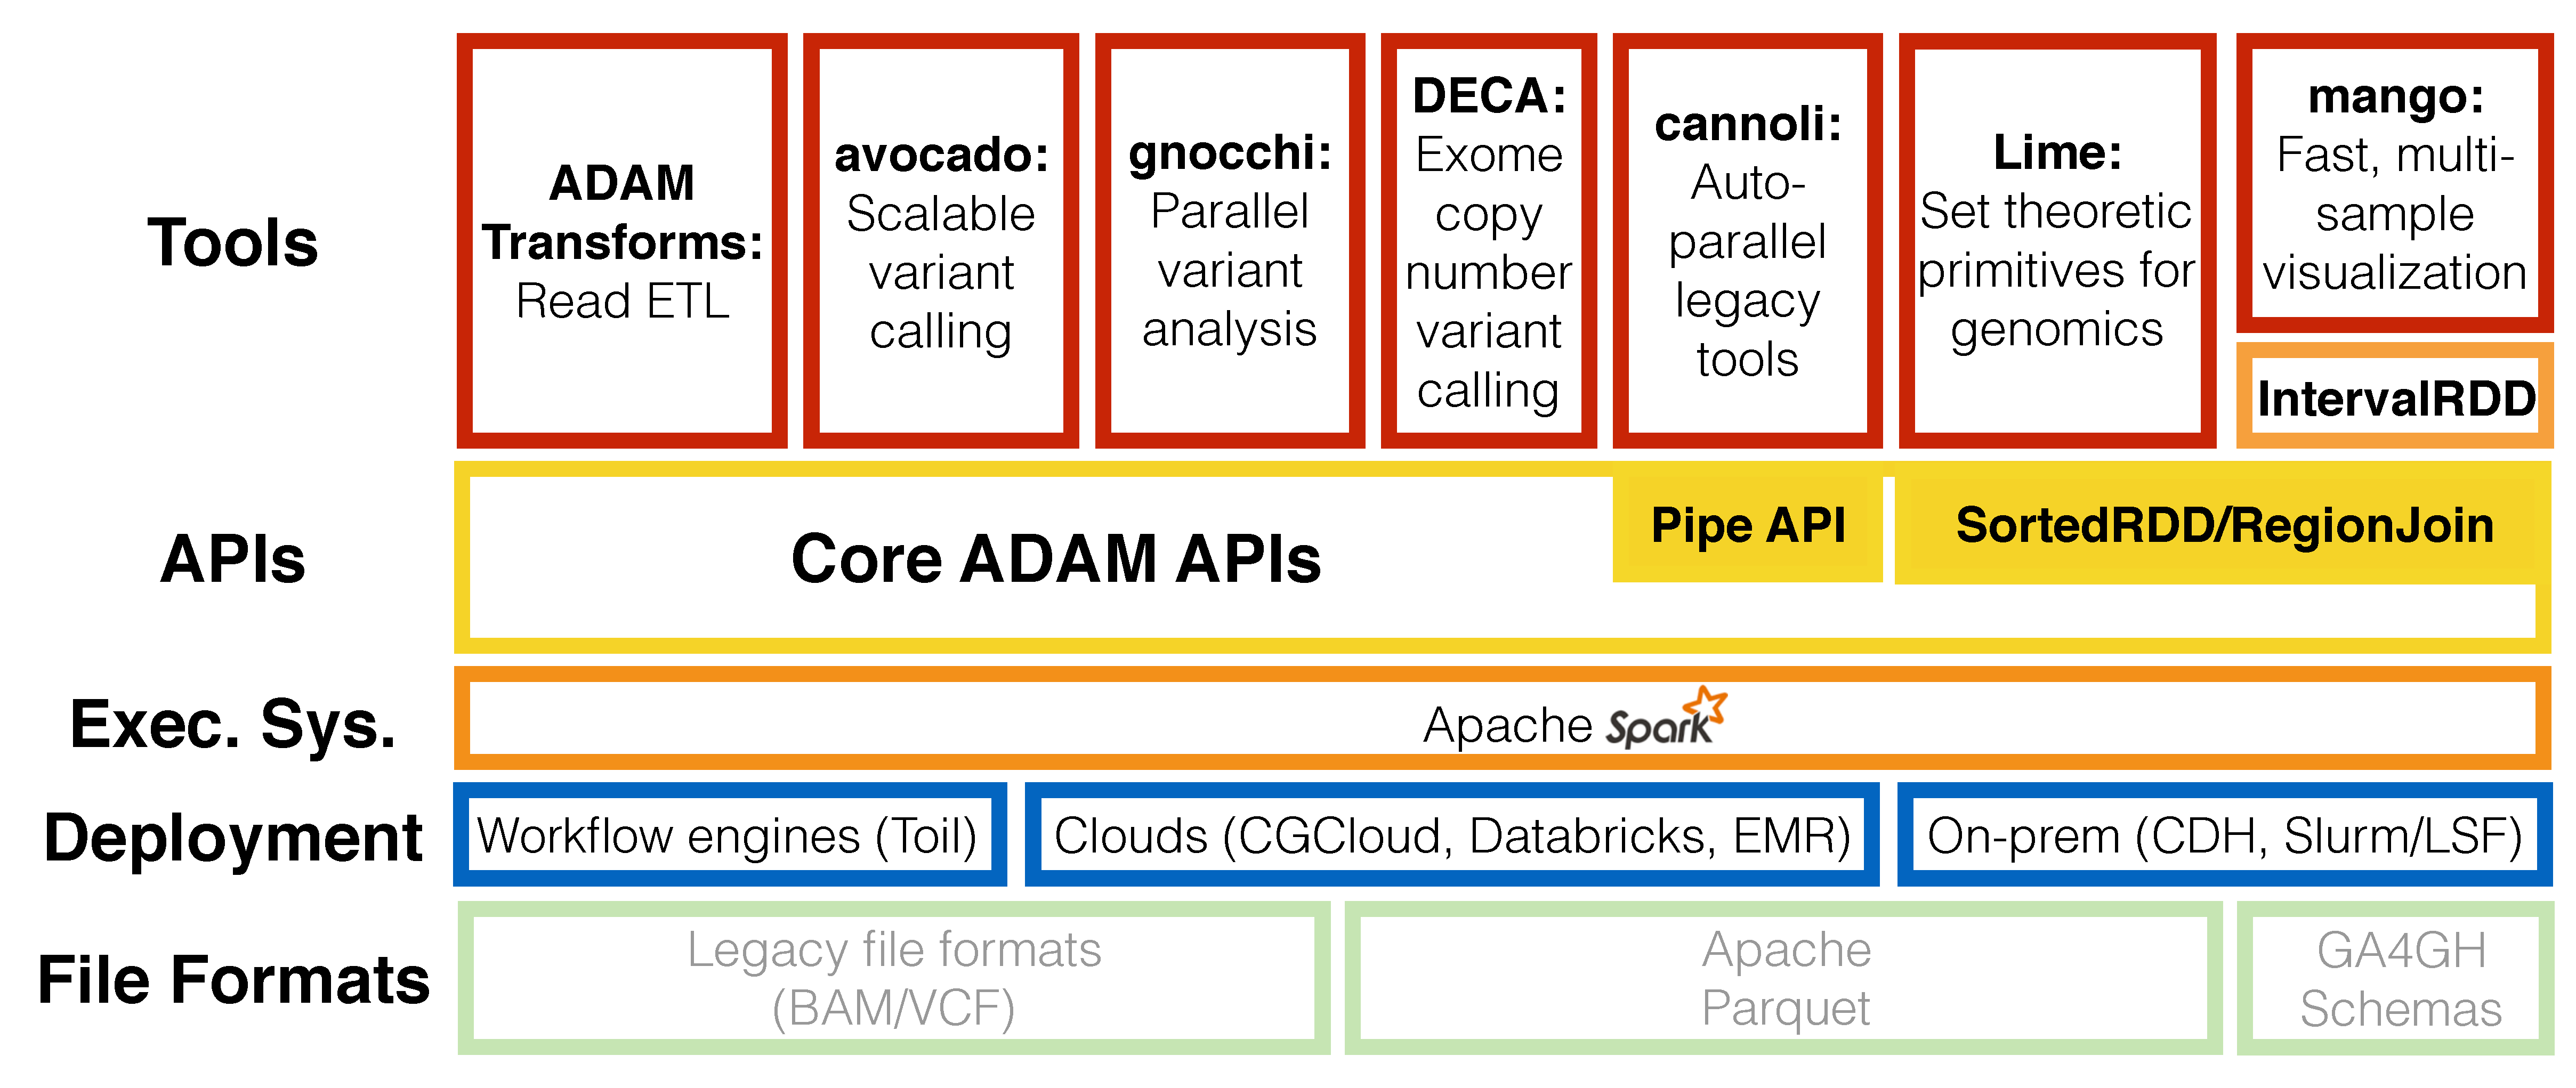
\includegraphics[width=0.95\linewidth]{graphs/bdgenomics-stack.pdf}
  \end{center}
  \caption{The Big Data Genomics ecosystem. Our work on \textsc{ADAM} has
    built a framework for scalable genomics using external projects like
    \textsc{Apache Spark}~\cite{zaharia12} and \textsc{Apache
      Parquet}~\cite{parquet}. On top of \textsc{ADAM}'s core APIs, we have
    built a broad ecosystem of tools~\cite{tu16, morrow17, linderman17}
    demonstrating how \textsc{Apache Spark} can accelerate genomic data
    analysis. To enable the reproducible use of \textsc{Apache Spark} in
    scientific data analysis workloads, we have contributed to novel,
    cloud-native workflow systems~\cite{vivian17}.}
  \label{fig:bdg}
\end{figure}

In this dissertation, we begin by describing the deluge of genomic data and the
tools that are used to process, manipulate, and store genomic data. In part two,
we then describe the requirements for a distributed genomic data analysis
framework and introduce \textsc{ADAM}'s architecture. Part three describes how
we built the \textsc{Cannoli}-\textsc{ADAM}-\textsc{Avocado} variant calling
pipeline on top of \textsc{ADAM}'s architecture, and the novel algorithms and
architectural refinements that were needed. We then validate the accuracy of
this pipeline in part four using ground truth datasets~\cite{zook15} and a large
scale sequencing project~\cite{mallick16}. We conclude by describing open
problems and future directions for this research, as well as the impact of the
Big Data Genomics/\textsc{ADAM} project.

\section{Economic Trends and Population Scale Sequencing}
\label{sec:economic-trends-population-scale}

The need for tools capable of processing large genomic datasets is precipitated
by the rise of popultation scale sequencing. While the raw data from a single
genome may be provide insight into the fitness of a single individual, genetic
data is most meaningful when viewed in aggregate across large cohorts.
For variants that do not have an obvious and severe pathogenic effect, our best
lens for understanding their impact from genomic data is through statistical
association testing. While genome wide association testing~(GWAS) has yielded
some successes, including prominent findings in neurogenetics~\cite{ripke14},
GWAS has faced several limitations. First, the association between genotype and
phenotype is often weak, unless the variant under study is strongly
pathogenic~\cite{shi16}. Additionally, few traits are truly Mendelian.
For complex traits, which are driven by the combined effect of multiple
genotypes~\cite{boyle17}, much heritability is explained through the complex
interaction of variants that impact regulatory regions. Modeling the effect of
non-coding changes is still an active area of work~\cite{weingarten14}.
Additionally, some diseases decompose into disease subtypes when studied in
aggregate. A strong example of this is acute myleoid leukemia~(AML): genomic
sequencing of germlines and tumors from a cohort of AML patients reveals
that AML is composed of eight or more genetic subtypes~\cite{aml13}. This
hinders classifying the impact of a single mutation, especially as some
gene mutations can be shared across disease subtypes.

These population scale sequencing projects have been enabled entirely by
technical innovation. While it cost more than \$100M to complete the data
acquisition for the Human Genome Project, the cost of sequencing a single
genome has dropped to under \$1,000~\cite{nhgri}. This has been driven by
continuous technical improvements by Illumina and competing sequencer vendors.
With the continued improvement of nanopore sequencing~\cite{jain17}, we may see
an additional precipitous drop in sequencing costs, as nanopore sequencers have
both lower capital and reagent costs relative to the Illumina sequencing
platform, but are currently limited in throughput and accuracy.

At the intersection of these two trends, population-scale sequencing has arisen.
The first population scale sequencing project was the 1,000 Genomes
project~\cite{1kg}, which collected a total data catalog of more than 75
terabytes~(TB) of data. Since then, sequencing projects have pushed beyond
petabyte-scale~(PB), with the 3PB catalog collected by The Cancer Genome
Atlas~(TCGA,~\cite{weinstein13}) and the 300PB data catalog collected by the
ExAC~\cite{lek16} project. While population-scale sequencing has largely been
done in academic settings to date, these sequencing projects are beginning
to move into industrial and medical settings. These include the collaboration
between the United Kingdom's Biobank, GlaxoSmithKline, and Regeneron to sequence
the 500,000 individuals in the UK Biobak~\cite{ukbiobank}, and the Geisenger
MyCode collaboration with Regeneron~\cite{carey16}.

\section{The Case for Distributed Computing for Genomic Analysis}
\label{sec:distributed-computing-for-genomics}

The rapid uptake of genome sequencing in academic, industrial, and clinical
settings is driving the total number of human genomes sequenced to double
approximately once every seven months~\cite{stephens15}. This far outpaces
Moore's law at its peak, and is a rate of increase approximately four times
greater than current estimates of Moore's law, which peg the doubling of
transistor counts to occur approximately every two years. As a result of
this growth in the volume of sequencing data, legacy tools are struggling to
handle genome-scale analyses across cohorts~\cite{schadt10, linderman17}.
We believe that distributed computing is a natural solution to these problems.

As asserted in the original GATK manuscript that proposed a single-node
MapReduce architecture for genomic data processing~\cite{mckenna10}, most
genomic analysis tasks map naturally to a share-nothing computing architecture.
Heavyweight genomic data analyses like alignment, variant calling, and
association testing either typically work on unaligned data, or are implemented
on a sorted stream traversing aligned data (the ``walker'' model). These
patterns either lack data dependencies~(unaligned reads, or analyses that look
at a single genomic locus), or have well defined spatial communication
patterns~(process data overlapping a given locus). These computations can
typically be paralellized with minimal communication. Additionally, many genomic
analysis queries map directly onto relational primitives which are implemented
in existing distributed data analysis platforms~\cite{armbrust15}. An example of
this is a genomic association test, which can be implemented as an aggregation
query.

To take full advantage of distributed computing, we believe that we need to do a
clean slate re-architecture of the genomic data processing infrastructure. In a
typical genomic processing pipeline, the analysis tools are typically designed
assuming a flattened stack running on a single node, or on a high performance
computing~(HPC)-style cluster with shared storage. These systems typically make
strong assumptions about the cost of making random accesses into a POSIX file
system, and present low level abstractions to users. While there have been
several attempts to retrofit legacy tools onto distributed
computing~(\textsc{CloudBurst}~\cite{schatz09}
and~\textsc{Crossbow}~\cite{langmead09}), these approaches have typically used
custom wrappers around \textsc{Apache Hadoop Streaming} and have been
non-general. There have also been several attempts to retrofit genomics-specific
file formats onto distributed query
architectures~(\textsc{SegPig}~\cite{schumacher14} and
\textsc{BioPig}~\cite{nordberg13}), but these implementations provide either
poor programming models or inefficient implementations. By doing a clean-slate
rearchitecture, we can eliminate architectural problems and provide better
user-facing query models with better performance.

\section{Mapping Genomics onto Distributed Computing using \textsc{ADAM}}
\label{sec:mapping-genomics-to-distributed-computing}

To address these problems, we propose \textsc{ADAM}, a comprehensive framework
for processing genomic data using the \textsc{Apache Spark} framework for
distributed computing. \textsc{ADAM} defines schemas for a full range of genomic
datatypes, which provides a data-indepent query model. These schemas form the
basis of a narrow waisted stack, which yields APIs that support both genomic
query and metadata management. By extending \textsc{ADAM} onto \textsc{Apache
  Spark SQL}, these APIs can be used across multiple languages. This extends the
power of distributed computing to bioinformatics users who are writing in the
Python or R languages, as opposed to previous tools that were centered either
around Java or the Pig scripting language~\cite{nordberg13, schumacher14}.

To demonstrate \textsc{ADAM}, we have built an end-to-end variant calling
pipeline. This pipeline includes distributed implementations of alignment, read
preprocessing, and variant calling. The pipeline can run end-to-end on a
$60\times$ coverage whole genome in under an hour, at a cost of $<$\$15 on
cloud computing. This pipeline provides results comparable to state-of-the-art
for single nucleotide variant~(SNV) calling, and high accuracy~(97\%) for
insertion and deletion~(INDEL) variant calling. Additionally, the alignment
step in this pipeline is implemented on top of a general interface for
parallelizing single-node genomics tools, which makes it possible to leverage
distributed computing without reimplementing a tool or developing custom shims,
unlike prior approaches~\cite{langmead09, schatz09}.

As a result, \textsc{ADAM} improves over conventional genomics tools by providing:

\begin{itemize}
\item Schemas which can support loading data from a large variety of formats.
\item High level, quasi-relational APIs for manipulating genomic data in both
  single node and cluster environments.
\item Parallel I/O across genomics file formats.
\item A simple API for parallelizing single node genomic tools with a minimal
  amount of code.
\end{itemize}

In the rest of this dissertation, we explain the design goals behind 
\textsc{ADAM}. By reviewing the architecture and implementation of
\textsc{ADAM}, we explain how these goals have shifted over time, informed by
our development experiences. We then demonstrate the \textsc{ADAM} architecture
through the \textsc{Cannoli} and \textsc{Avocado} tools, which implement the
\textsc{Big Data Genomics} variant calling pipeline.

\chapter{Background and Related Work}
\label{chap:background}

While there are many ways to collect and then process genomic data, this
dissertation focuses on the ``genome resequencing'' pipeline. In resequencing,
we start with a known genome assembly, and identify the edits between an
individual genome and the genome assembly for their species. In practice, a
genome resequencing analysis pipeline will typically take short sequenced
reads~(100-300 base pairs, bp), align them to the reference genome, perform
preprocessing on the reads to eliminate errors, and then probabilistically
identify true variation from the reads. In this chapter, we will start by
describing how the reads are sequenced~(\S\ref{sec:genome-sequencing}) and
analyzed~(\S\ref{sec:genomic-analysis}). We will then dive deeper into the
representations of genomic data~(\S\ref{sec:genomic-data-representations}),
and the architectures used to process this
data~(\S\ref{sec:genomic-architectures}). Then, we will review the variant
identification algorithms~(\S\ref{sec:variant-calling-approaches}). Finally,
we will discuss the emergence of commodity distributed computing
frameworks~(\S\ref{sec:distributed-computing}) and how researchers have
approached parallelizing genome resequencing
pipelines~(\ref{sec:distributed-genome-analysis})

\section{Genome Sequencing Technologies}
\label{sec:genome-sequencing}

Since the Human Genome Project released the first assembly of the Human genome
in 2001~\cite{lander01}, biochemical and algorithmic advancements have enabled
the broad analysis of biological phenomena through sequencing. Although the
full spectrum of sequencing-based analyses is beyond the scope of this
manuscript, these assays rely on encoding a biological phenomena into DNA, which
is then sequenced and analyzed statistically. In this section, we provide a
brief introduction to the sequencing process before focusing on the algorithmic
approaches used to determine the sequence variants in a single genome. We will
focus on data generated using Illumina sequencers, as this sequencing modality
is commonly used for genomic variant detection.

To run a sequencing assay, we start by preparing a sequencing library, which is
then run through a sequencer. This stage creates genomic ``reads'', which
include a string of bases~(in the A, C, G, T alphabet used by DNA) along with
estimates of the probability that a single base was read correctly. The library
preparation stage converts the biological sample into DNA fragments, which we
can sequence. In the simplest case~(sequencing a genome), we start by extract
DNA from a collection of cells. We then slice the long DNA strands into shorter
fragments, before selecting fragments of a certain length (``size selection'').
The size of fragments collected depends on both the sequencing instrument that
is being used, and the biological assay being conducted. Common variants on this
process include exome sequencing (where we start from DNA, but select the regions
of the genome that encode genes before fragmenting and size selecting reads),
RNA-seq (where we start by converting single stranded RNA into DNA, which is
then fragmented and size selected, see~\cite{mortazavi08}). There are many
biological assays that can be encoded as sequencing and a full review is beyond
the scope of this manuscript; we refer readers to Soon et al~\cite{soon13} for a
more comprehensive overview.

Many modern variant analysis pipelines use paired reads from Illumina
sequencers. Depending on the specific sequencer model and chemistry, Illumina
sequencers support read lengths ranging from 75 to 300 bases. All reads from an
Illumina sequencer have the same length, as the length of the read is determined
by the number of cycles that the sequencer is run. ``Paired''  means that we
generate two reads from each DNA fragment; we read one read from each strand of
the DNA, with the two reads coming from opposite ends of the DNA fragment.
In a conventional sequencing libraries, the DNA fragments include bases that are
not sequenced; these bases are typically referred to as the ``insert'', and the
number of bases not sequenced (``insert size'') are controlled through the
size selection process. For example, if we wanted to prepare a paired sequencing
library where the read length was 250 bases with an average insert size of 500
bases, we would select all fragments that were approximately 1,000 bases long
(250 bases for the first read, approximately 500 bases between the first and
second read, 250 bases for the second read). There are many variants on this
process, including those that have negative insert sizes, and ``mate pair''
libraries that have very long insert sizes~\cite{mardis13}. Additionally,
library preparation varies tremendously between sequencing vendors. For long
read sequencers such as the Pacific Biosciences sequencers~\cite{eid09} or
the Oxford Nanopore sequencers~\cite{clarke09}, the libraries include long DNA
fragments~(>5,000 bases) that generate a single, full length read.

Illumina sequencers generate reads through a sequencing-by-synthesis approach.
In this process, flourescent dyes are attached to the DNA bases. The sequencer
then takes an image of the dyes, which is then converted into the called bases.
This process runs for a fixed number of cycles, which sets the length of the
sequenced reads. To ensure that the bases from a single read show up in the same
locations in the image betwen cycles, the ends of the reads are attached to
knobs that protrude from glass plates. At the end of each cycle, the dyes are
washed off of the end of the read, which exposes the next base in the read for
a new round of dyes to attach to. The probability that a base was sequenced
correctly is determined by looking at the color and intensity of the base on
the captured image. Illumina platforms are susceptible to single base substition
errors, which occur to a 0.5--2\% of bases. This error rate is problematic for
variant calling, as we expect a variant to occur at one in every one thousand
bases.

Many of the analyses that use reads generated from Illumina sequencers are
analyzed with mapping-based approaches. In this class of approaches, we rely on
the existence of a ``reference genome'' for an organization. This is a curated
dataset that consists of the DNA sequences for all of the chromosomes in the
genome of a species. For humans, the first reference genome was generated
through the Human Genome Project~\cite{lander01}. New genome references are
released every several years and include corrections to prior reference genomes
and new assemblies for areas of the genome that are hard to sequence (typically
caused by the genome being highly repetitive in a single area). The most recent
release of the human genome~(GRCh38, see~\cite{church15}) was released at the
end of 2014. A reference genome defines a two dimensional coordinate space, with
one coordinate selecting the chromosome and the second coordinate defining the
position on this chromosome.

\section{Genomic Analysis Tools and Architectures}
\label{sec:genomic-analysis}

In a mapping-based approach, the reads are mapped to a location of the reference
genome, and then locally aligned. Mappers query subsequences from a read against
an index built from the reference genome. This process will identify the ranges
in the genome that the read could plausibly align to. Once these ranges have
been identified, the mapper will then locally align the read sequence against
the genomic sequences from these ranges, using an edit calculation algorithm such
as Smith-Waterman~\cite{smith81}, Ukkonen's algorithm~\cite{ukkonen85}, or a
pairwise sequence alignment Hidden Markov Model~(HMM,~\cite{durbin98}). Widely
used mappers include \textsc{BWA}~\cite{li09}, which builds an index using the
Burrows-Wheeler transform~\cite{burrows94}; \textsc{Bowtie}~\cite{langmead09},
which builds an FM-index~\cite{ferragina00}; and \textsc{SNAP}~\cite{zaharia11},
which builds a hash-based index. Several projects have applied hardware acceleration
to alignment, including \textsc{cloud-scale-bwamem}~\cite{chen15, chen16}, Ahmed
et al~\cite{ahmed15}, and unpublished work out of Microsoft
Azure~\cite{msr16}.

Variant calling is one such mapping-based approach. To identify variants between
the genomes of two individuals, we compute the difference of each individual
against the reference genome, and then compute the transitive difference between
the two individuals. To compute the variations between a single individual and
the reference, we start by aligning the reads to the reference genome. From
here, we can then look at each site in the genome to see if there are reads that
support an sequence edit. This is typically done by applying a statistical model
to the reads that looks at the base error probabilities attached to the reads
that contain the reference sequence and the reads that contain the proposed
sequence variant. Examples of the models used include the \textsc{SAMTools
mpileup} variant caller~\cite{li11}, and the \textsc{GATK
UnifiedGenotyper}~\cite{depristo11}. However, the aligned reads frequently
include errors that can lead to incorrect variant calls. To eliminate these
errors, we rely on several preprocessing stages that are run between mapping and
variant calling. In this paper, we will focus on three preprocessing stages:
duplicate removal, local realignment, and base quality score recalibration.
The variant calling pipeline has been targeted for hardware acceleration in the
unpublished Edico \textsc{DRAGEN} processor~\cite{dragen}.

The duplicate removal stage identifies DNA fragments that were duplicated during
library preparation. If we are starting from a biological sample that contains
very little DNA, we will commonly use a polymerase chain reaction~(PCR) during
library preparation. This reaction will take our input DNA and replicate it,
thereby increasing the amount of DNA that we can provide to the sequencer.
However, as part of the PCR process, some fragments will be excessively
replicated. This can lead to a single fragment being replicated 100 times. If
this fragment contains a sequence variant or a sequence that is susceptible to
being sequenced incorrectly, this can bias the genomic region where the read is
located and lead to an incorrect variant being identified.

Local realignment is typically run after duplicate marking and addresses an
issue inherent to the mapping process. Specifically, if there are larger
sequence variants (e.g., multi-base insertions or deletions) into a read, the
mapping process will commonly identify the correct genomic region that a read
should map to, but will locally misalign the read relative to other reads that
contain the same underlying sequence variant~\cite{depristo11}. During local
realignment, we start by identifying all possible insertion/deletion~(INDEL)
variants in our reads. For every region that contains an INDEL, we then look
at the reads that map to that region. We identify the most common sequence
variant in the set of reads and rewrite the local read alignments ensure that
all reads that contain a single sequence variant are aligned with a consistent
representation. This step is necessary because the algorithms used to compute
the pairwise alignment of two sequences are fundamentally
probabilistic~\cite{durbin98, smith81, ukkonen85}, which can lead to
inconsistent representations for equivalent sequence edits~\cite{li14}.

The final preprocessing stage is base quality recalibration. As mentioned
earlier, when the reads are sequenced, the sequencer estimates the probability
that a single base was sequenced in error from the color and intensity of the
light emitted from the floursecent dye. In practice, sequencing errors correlate
with various factors, including sequence context (the bases around the base that
is being sequenced) and the stage when the base was sequenced (due to errors
with the sequencing chemistry during that sequencing cycle). The base quality
recalibration stage associated each base with error covariates, and then
calculates the empirical error rate for the bases in that covariate by measuring
the frequency with which bases in that covariate mismatch the reference genome.
These error rates are then converted back into probabilites, which replace the
probabilities attached to the reads.

We have chosen to focus on the read preprocessing algorithms used for variant
calling for several reasons. First and foremost, variant calling is the most
widely used analysis across contemporary genomics, and is a core part of large
population-scale studies such as the 1,000 Genomes Project~\cite{1kg12, 1kg},
the Exome Aggregation Consortium~\cite{lek16}, and The Cancer Genome
Atlas~\cite{weinstein13}. Additionally, the read preprocessing stages are
tremendously computationally expensive. For a single human genome sequenced with
an average of 60 reads covering each genomic position, it takes over 160 hours
to align the reads, preprocess the reads, and call variants, with approximately
110 of the hours spent preprocessing the reads. Finally, implementations of thes
algorithms are available as part of the widely used \textsc{Genome Analysis
Toolkit}~\cite{mckenna10, depristo11} and \textsc{ADAM}~\cite{massie13,
nothaft15} libraries.

\subsection{Genomic Data Representations}
\label{sec:genomic-data-representations}

Currently, genomic data are stored in a myriad of file formats that largely
descend from formats that were developed during the 1,000 Genomes
project~\cite{1kg}. Some of these formats are much older; many genomic feature
file formats descend from the development of the University of California,
Santa Cruz's (UCSC) Genome Browser~\cite{kent02}, which was developed as part
of the Human Genome Project~\cite{lander01}, and informal specificiations for
the FASTQ~\cite{cock09} and FASTA formats date back to at least the nineties,
through their use in the \textsc{phred}~\cite{ewing98} and
\textsc{FASTA}/\textsc{FASTP}~\cite{pearson90} tools.

The file formats developed during the 1,000 Genomes project stored high
throughput sequencing data in tab separated value~(TSV) files. These
formats included the \textsc{Sequence Alignment/Mapping}~(SAM)
format~\cite{li09}, which represents genomic reads and the \textsc{Variant Call
  Format}~(VCF) format~\cite{danecek11}, which was defined to store variants
and genotypes. The 1000 Genomes project also made significant use of the
TSV \textsc{Browser Extensible Data}~(BED) format for storing genomic feature
data. While the BED format had been introduced earlier, the introduction of
\textsc{BEDTools}~\cite{quinlan10} during the 1,000 Genomes Project drove
the further use of the BED format. A plethora of textual file formats exist for
storing genomic feature data, such as the \textsc{NarrowPeak} format, a
specialized variant of BED that is used by the \textsc{MACS}~\cite{zhang08}
tool; the \textsc{IntervalList} format, which is used extensively by the
\textsc{GATK}~\cite{depristo11}; and the \textsc{General Feature Format}~(GFF),
which is used extensively in sequence annotation projects like the Sequence
Ontology~\cite{eilbeck05}.

Over time, some of these formats have been replaced by binary variants that
provide improved compression and performance. SAM has been largely replaced
in practice by the \textsc{Binary Alignment/Mapping}~(BAM) format, and the
binary VCF~(BCF) has entered use for storing variant data. In practice,
textual file formats are still broadly used for storing variant and feature
data, but they are often compressed using a block-compressed codec, such as
BGZF~\cite{li11tabix}. There has been significant research towards developing
compressed storage formats for alignment data~\cite{kozanitis11, fritz11}.
The CRAM codec has achieved the broadest use, and uses reference-based
compression to avoid storing read sequence that matches the reference genome.
Additionally, CRAM can apply lossy compression schemes---such as base quality
score binning---to achieve further compression.

\subsection{Genomic Analysis Architectures}
\label{sec:genomic-architectures}

Although there exist myriad tools for analyzing genomic data, very few tools
espouse a systematic architecture for traversing and processing genomic data.
Instead, most tools are built around a UNIX-inspired philosophy that asserts
that ``a tool should do a single task well''~\cite{rodriguez11}, and simply
traverse a stream of data. The most promiment example of a genomic analysis
architecture is the quasi-map-reduce architecture employed by the legacy
versions of the GATK~\cite{mckenna10}. This architecture uses an iterator-based
model called a ``walker'' to traverse over data aligned to reference genome
coordinates. The ``map-reduce'' nature of this API describes how chunks of
genome aligned data can be parallelized, with a reduce operation supported
for summarizing tables of data across threads, as is used for combining
Base Quality Score Recalibration~(BQSR) tables. While this API could
conceptually be used in a distributed setting, the GATK has historically
only run as a multithreaded application on a single node. Instead,
multi-node execution was provided through the \textsc{Queue}~\cite{depristo11}
workflow manager.

While the UNIX-like design philosophy espoused by many bioinformatics tools
allows for the creation of tools with well defined boundaries, this seems to be
fundamentally at odds with the reality of complex genomics workflows, where many
tools must be cascaded one-after-the-other. As a result, genomics has embraced
workflow management as an alternate paradigm, where tools are composed into an
abstract workflow, which is then executed by the management system. A popular
early system was the \textsc{Galaxy}~\cite{goecks10} tool, which provided a
graphical user interface for defining workflows and tool invocations. Recently,
a set of novel workflow management systems have been developed, such as
\textsc{Toil}~\cite{vivian17}, \textsc{NextFlow}~\cite{ditommaso17},
\textsc{Rabix}~\cite{kaushik16}, \textsc{Cromwell}~\cite{cromwell},
and \textsc{Cuneiform}~\cite{brandt15}. These systems exploit many-task
parallelism, and are well suited to analyses where a cohort of many samples
should be analyzed independently by sample. These systems differ in their
approach to expressing workflows. Several efforts to standardize workflow
descriptions have emerged, with the most prominent community being around the
\textsc{Common Workflow Language}~\cite{cwl}. \textsc{Toil} is implemented as
a Python library that allows for workflows to be natively defined in Python,
and can also run workflows written in CWL, or in \textsc{Cromwell}'s WDL
dialect. \textsc{Rabix} executes CWL. \textsc{NextFlow} and \textsc{Cuneiform}
both take a clean slate approach to implementing a workflow language, using
dataflow and functional approaches to describe workflows.

\subsection{Variant Calling Approaches}
\label{sec:variant-calling-approaches}

The accuracy of insertion and deletion~(INDEL) variant discovery has been improved by the development
of variant callers that couple local reassembly with haplotype-based statistical models to recover INDELs
that were locally misaligned~\cite{albers11}. Now, several prominent variant callers such as the Genome
Analysis Toolkit's~(GATK) \textsc{HaplotypeCaller}~\cite{depristo11}, \textsc{Scalpel}~\cite{narzisi14}, and
\textsc{Platypus}~\cite{rimmer14}. Although haplotype-based methods have enabled more accurate INDEL
and single nucleotide polymorphism~(SNP) calls~\cite{bao14}, this accuracy comes at the cost of
end-to-end runtime~\cite{talwalkar14}. Several recent projects have been focused on improving
reassembly cost either by limiting the percentage of the genome that is reassembled~\cite{bloniarz14} or
by improving the performance of the core algorithms used in local reassembly~\cite{rimmer14}.

The performance issues seen in haplotype reassembly approaches derives from the high asymptotic
complexity of reassembly algorithms. Although specific implementations may vary slightly, a typical
local reassembler performs the following steps:

\begin{enumerate}
\item A de Bruijn graph is constructed from the reads aligned to a region of the reference genome,
\item All valid paths~(\emph{haplotypes}) between the start and end of the graph are enumerated,
\item Each read is realigned to each haplotype, typically using a pair Hidden Markov Model~(HMM,
see Durbin et al~\cite{durbin98}),
\item A statistical model uses the read$\leftrightarrow$haplotype alignments to choose the haplotype pair
that most likely represents the variants hypothesized to exist in the region, 
\item The alignments of the reads to the chosen haplotype pair are used to generate statistics that are
then used for genotyping.
\end{enumerate}

In this paper, we focus on improving the algorithmic efficiency steps one through three of the local reassembly problem.
We do not focus algorithmically on accelerating stages four and five, as there is wide
variation in the algorithms used in stages four and five. However, we do provide an parallel
implementation of a widely used statistical model for genotyping~\cite{li11}. Stage one (graph
creation) has approximately $\mathcal{O}(r l_r)$ time complexity, and stage two (graph elaboration) has
$\mathcal{O}(h \max(l_h))$ time complexity.
The asymptotic time cost bound of local reassembly comes from stage three, where cost is $\mathcal{O}(h r l_r
\max(l_h))$, where $h$ is the number of haplotypes tested in this region, $r$ is the number of reads aligned to this region, $l_r$ is the read length,
and $\min(l_h)$ is the length of the
shortest haplotype that we are evaluating. This complexity comes from realigning $r$ reads to $h$
haplotypes, where realignment has complexity $\mathcal{O}(l_r l_h)$. Note that the number of
haplotypes tested may be lower than the number of haplotypes reassembled. Several tools
(see Depristo et al~\cite{depristo11} and Garrison and Marth~\cite{garrison12}) allow users to limit the number of haplotypes evaluated to improve
performance. For simplicity, we assume constant read length. This is a reasonable assumption as many of the variant
callers discussed target Illumina reads that have constant length, unless the reads have been trimmed
during quality control.

In this paper, we introduce the indexed de Bruijn graph and demonstrate how it can be used to
reduce the asymptotic complexity of reassembly. An indexed de Bruijn graph is identical to a
traditional de Bruijn graph, with one modification: when we create the graph, we annotate each
$k$-mer with the index position of that $k$-mer in the sequence it was observed in. This simple addition
enables the use of the indexed de Bruijn graph for $\Omega(n)$ local sequence alignment with
canonical edit representations for most edits. This structure can be used for both sequence alignment and
assembly, and achieves a more efficient approach for variant discovery via local reassembly.
To further improve the efficiency of this approach, we demonstrate in~\S\ref{sec:implementation}
how we can implement the canonicalization scheme that we demonstrate using indexed de Bruijn
graphs without constructing a de Bruijn graph that contains both sequences.

Current variant calling pipelines depend heavily on realignment based approaches for accurate
genotyping~\cite{li14}. Although there are several approaches that do not make explicit use of reassembly,
all realignment based variant callers use an algorithmic structure similar to the one described
above. In non-assembly approaches like \textsc{FreeBayes}~\cite{garrison12}, stages
one and two are replaced with a single step where the variants observed in the reads aligned to a given
haplotyping region are filtered for quality and integrated directly into the reference haplotype in that region.
In both approaches, local alignment errors~(errors in alignment \emph{within} this region) are corrected
by using a statistical model to identify the most likely location that the read could have come from, given
the other reads seen in this area.

Although the model used for choosing the best haplotype pair to finalize realignments to varies between
methods~(e.g., the GATK's \textsc{IndelRealigner} uses a simple log-odds model~\cite{depristo11}, while
methods like \textsc{FreeBayes}~\cite{garrison12} and \textsc{Platypus}~\cite{rimmer14} make use of richer
Bayesian models), these methods require an all-pairs alignment of reads to candidate
haplotypes. This leads to the runtime complexity bound of $\mathcal{O}(h r l_r \min(l_h))$,
as we must realign $r$ reads to $h$ haplotypes, where the cost of realigning
one read to one haplotype is $\mathcal{O}(l_r \max(l_h))$, where $l_r$ is the read length~(assumed to be
constant for Illumina sequencing data) and $\max(l_h)$ is the length of the longest haplotype. Typically,
the data structures used for realignment~($\mathcal{O}(l_r \max(l_h))$ storage cost) can be reused.
These methods typically retain \emph{only} the best local realignment per read per haplotype, thus
bounding storage cost at $\mathcal{O}(h r)$.

For non-reassembly based approaches, the cost of generating candidate haplotypes is $\mathcal{O}(r)$,
as each read must be scanned for variants, using the pre-existing alignment. These variants are typically
extracted from the CIGAR string, but may need to be normalized~\cite{li14}. de Bruijn graph based 
reassembly methods have similar $\mathcal{O}(r)$ time complexity for building the de Bruijn
graph as each read must be sequentially broken into $k$-mers, but these methods have a different
storage cost. Specifically, storage cost for a de Bruijn graph is similar to $\mathcal{O}(k
(l_{\text{ref}} + l_{\text{variants}} + l_{\text{errors}}))$, where $l_{\text{ref}}$ is the length of the reference
haplotype in this region, $l_{\text{variants}}$ is the length of true variant sequence in this region, 
$l_{\text{errors}}$ is the length of erroneous sequence in this region, and $k$ is the $k$-mer size. In
practice, we can approximate both errors and variants as being random, which gives $\mathcal{O}(k
l_{\text{ref}})$ storage complexity. From this graph, we must enumerate the haplotypes present in the
graph. Starting from the first $k$-mer in the reference sequence for this region, we perform a depth-first
search to identify all paths to the last $k$-mer in the reference sequence. Assuming that the graph is
acyclic~(a common restriction for local assembly), we can
bound the best case cost of this search at $\Omega(h \min l_h)$.

The number of haplotypes evaluated, $h$, is an important contributor to the algorithmic complexity of
reassembly pipelines, as it sets the storage and time complexity of the realignment scoring phase, the
time complexity of the haplotype enumeration phase, and is related to the storage complexity of the
de Bruijn graph. The best study of the complexity of assembly techniques was done by Kingsford
et al.~\cite{kingsford10}, but is focused on \emph{de novo} assembly and pays special attention to
resolving repeat structure. In the local realignment case, the number of haplotypes identified is determined
by the number of putative variants seen. We can na\"{i}vely model this cost with \eqref{eq:haplotypes},
where $f_v$ is the frequency with which variants occur, $\epsilon$ is the rate at which bases are
sequenced erroneously, and $c$ is the coverage (read depth) of the region.

\begin{align}
\label{eq:haplotypes}
h \sim f_v l_{\text{ref}} + \epsilon l_{\text{ref}} c
\end{align}

This model is na\"{i}ve, as the coverage depth and rate of variation varies across sequenced datasets,
especially for targeted sequencing runs~\cite{fang14}. Additionally, while the $\epsilon$ term models the
total number of sequence errors, this is not completely correlated with the number of \emph{unique}
sequencing errors, as sequencing errors are correlated with sequence context~\cite{depristo11}. Many
current tools allow users to limit the total number of evaluated haplotypes, or apply strategies to minimize
the number of haplotypes considered, such as filtering observed variants that are likely to be sequencing
errors~\cite{garrison12}, restricting realignment to INDELs~(\textsc{IndelRealigner},~\cite{depristo11}), or
by trimming paths from the assembly graph. Additionally, in a de Bruijn graph, errors in the
first $k$ or last $k$ bases of a read will manifest as spurs and will not contribute paths through the graph. We provide~\eqref{eq:haplotypes} solely as a motivating
approximation, and hope to study these characteristics in more detail in future work.

\section{Distributed Computing Platforms}
\label{sec:distributed-computing}

Google described the use of large clusters of commodity computers in their
\textsc{MapReduce} system~\cite{dean04, dean08} in 2004. Since then, there has
been a surge of activity focusing on the development of distributed data
analysis tools. In the open source world, this has spawned the \textsc{Apache
  Hadoop} project~\cite{hadoop}, which started as a open source reimplementation
of Google's \textsc{MapReduce}. \textsc{Hadoop} led to the development of
scripting languages like \textsc{Pig}~\cite{olston08}, query systems like
\textsc{Hive}~\cite{thusoo09}, and resource management frameworks like
\textsc{YARN}~\cite{vavilapalli13} and \textsc{Mesos}~\cite{hindman11}. While
traditional map-reduce platforms were well suited to extract, transform,
load~(ETL) pipelines that made a single pass over a large dataset, they were
a poor fit to ``advanced analytics'' applications---like machine learning, or
graph processing---that made several passes over a dataset. This was due to
their reliance on the output of every computational phase being written to
disk to ensure fault tolerance. A new set of distributed data processing tools
were designed to address this problem by storing data in memory, and relying
on different models for fault resilience. These systems include
\textsc{Spark}~\cite{zaharia10, zaharia12} and \textsc{Flink}~\cite{carbone15}.
Additionally, a set of highly efficient query engines came out, such as
\textsc{Cloudera Impala}~\cite{kornacker15} and \textsc{Spark
  SQL}~\cite{armbrust15}.

\subsection{Distributed Genomic Analysis Tools}
\label{sec:distributed-genome-analysis}

Genomics tools that leverage commodity distributed computing have typically
taken one of two approaches: either they wrap a single-node tool so that it can
be parallelized using a distributed computing framework, or they define a
distributed query model for a single area/tool of focus. Beyond these two
approaches, some tools have been built on distributed computing technologies
from the HPC ecosystem. Additionally, cloud-friendly workflow management
systems have entered broad usage.

There have been three waves of development focused on integrating single-node
tools with distributed computing platforms. The first wave of development used
\textsc{Apache Hadoop Streaming} as a simple mechanism for parallelising tools
that had well defined chunking patterns. Examples of this approach include the
\textsc{CloudBurst} aligner~\cite{schatz09}, which parallelized the
\textsc{RMAP} aligner~\cite{smith08}, and
\textsc{CrossBow}~\cite{langmead09crossbow}, which integrates the
\textsc{Bowtie}~\cite{langmead09bowtie} aligner with the
\textsc{SoapSNP}~\cite{li09snp} variant caller. The second wave of approaches
built more fully featured applications on top of the \textsc{Apache Hadoop}
framework that did not just rely on the streaming APIs. These applications
include the \textsc{SEAL}~\cite{pireddu11} aligner, which extracted the
\textsc{BWA}~\cite{li09} aligner into a Python library which was executed
on the \textsc{PyDoop}~\cite{leo10} bindings for \textsc{Hadoop};
\textsc{BigBWA}~\cite{abuin15}, which parallelizes \textsc{BWA}~\cite{li09}
using the Java Native Interface~(JNI) on top of \textsc{Apache Hadoop}; and
\textsc{Halvade}~\cite{decap15}, which parallelized the complex dataflow in
the \textsc{GATK}~\cite{depristo11} using \textsc{Apache Hadoop}. The third
wave of wrappers has been built around \textsc{Apache Spark} and includes
\textsc{SparkBWA}~\cite{abuin16}, a successor to \textsc{BigBWA}~\cite{abuin15},
\textsc{CloudScale-BWA MEM}~\cite{chen16}, which parallelizes
\textsc{BWA} through the JNI, with the ability to support \textsc{FPGA}
acceleration; and \textsc{SparkGA}~\cite{mushtaq17}, which uses a similar
approach as \textsc{Halvade} to parallelize the \textsc{GATK}, but is
implemented on \textsc{Spark}.

Several tools have implemented genomic analyses directly on top of distributed
analysis tools from the \textsc{Apache Hadoop} and \textsc{Spark} ecosystem.
Many of these tools build on top of the \textsc{Hadoop-BAM}
library~\cite{niemenmaa12}, which provides \textsc{Hadoop}-compatible parallel
I/O libraries. The first generation of tools built query models for accessing
genomic data through the \textsc{Pig}~\cite{olston08} scripting language.
This was implemented in two separate tools: \textsc{BioPig}~\cite{nordberg13}
and \textsc{SeqPig}~\cite{schumacher14}. Additionally, the \textsc{OpenCB}
project has built \textsc{Hadoop}-based tools for manipulating genomic data via
the \textsc{hpg-bigdata} project~\cite{opencb}. Recent work has moved on to
\textsc{Apache Spark}. Beyond \textsc{ADAM} and the \textsc{Big Data Genomics}
ecosystem, \textsc{Spark} has been used in the
\textsc{SparkSeq}~\cite{wiewiorka14} and \textsc{VariantSpark}~\cite{obrien15}
tools. \textsc{SparkSeq} is geared towards RNA-seq analysis, and has been
paired with \textsc{SparkBwa}~\cite{abuin16} to build the
\textsc{Falco}~\cite{yang16} single-cell RNA-seq pipeline which runs end-to-end
on \textsc{Apache Spark}. \textsc{VariantSpark} includes novel methods for
statistically analyzing genotype data on \textsc{Spark}, including an efficient
implementation of random forests for wide-but-flat genomic data. There is
increasing adoption of \textsc{Apache Spark} in genomics, with two large
unpublished projects coming out of the Broad Institute. The first is the fourth
edition of the \textsc{GATK}~\cite{gatk4}, which is reimplemented on
\textsc{Spark}. The second project is \textsc{Hail}~\cite{hail}, which is a
reimplementation of the \textsc{PLINK} population genomics~\cite{purcell07}
toolkit on \textsc{Spark}.

We do not extensively discuss non-resequencing pipelines for de novo genome
assembly in this dissertation, but genome assembly has different access patterns
that are more amenable to HPC-styled distributed implementations. Specifically,
since de novo assembly operates on highly connected graphs, efficiently mapping
de novo assembly to a graph-parallel framework like
\textsc{GraphX}~\cite{gonzalez14} is difficult. The \textsc{ABySS}
assembler~\cite{simpson09} uses the Message Passing Interface~(MPI) to
parallelize genome assembly across an HPC cluster. A new and exciting avenue
of work is using HPC systems that support a parallel global address space~(PGAS)
and Remote Direct Memory Access~(RDMA) to achieve extremely fine grained
parallelism~\cite{georganas14, georganas15hipmer, georganas15meraligner,
  georganas17}.

\part{Architecture and Infrastructure}

\chapter{Design Principles for Scalable Genomics}
\label{chap:design}

When we started designing \textsc{ADAM} in 2013, \textsc{Apache Spark} was still
in early development, and few organizations were actively working with massive
genomics data sets. At the time, we believed that the major pain points in
working with large scale genomics datasets centered around low-level APIs that
made it difficult to represent complex genomic data manipulations and the use of
file formats that were difficult to access in parallel and that had imprecise
specifications. This led to the initial goals for the \textsc{ADAM} project:

\begin{itemize}
\item Provide clean APIs for writing large scale genomic data analyses
\item Raise abstraction by centering data manipulation around schemas instead
  of file formats
\item Allow these APIs to be exposed across commonly used languages
\item Efficiently execute non-reference oriented query patterns
\end{itemize}

To achieve these goals, we designed a decoupled, stack-oriented architecture
that was centered around schemas that provided a logical view over the genomic
data that was being manipulated. This architecture was implemented on top of
\textsc{Apache Spark}'s RDD APIs, and provided the user with a distributed
collection of genomic data which were encoded in \textsc{Apache
  Avro}~\cite{avro}. This allowed for queries to be described at a high level
through \textsc{Spark}'s RDD APIs, which would execute the queries rapidly by
running parallel scans over the data. Over time, our goals grew in scope to
include:

\begin{itemize}
\item Support coordinate-space joins with genomic data
\item Support exploratory data analysis on genomic datasets
\item Allow people to reuse their existing genomic analysis tools on Spark with
  minimal modifications
\end{itemize}

Because of \textsc{ADAM}'s decoupled architecture, we were able to easily
enhance \textsc{ADAM} to support these query patterns. By refactoring how
\textsc{ADAM} tracked data partitioning, the coordinate-space
joins~(\S\ref{sec:query-patterns}) and the \textsc{pipe} API for supporting
legacy genomics tools~(\S\ref{sec:query-patterns}) were added to \textsc{ADAM}'s
core APIs. The \textsc{Mango} project enhanced \textsc{ADAM}'s ability to run
interactive queries against genomic data by improving support for pushing down
ranged predicates to disk~\cite{tu16} and by adding a spatial- and temporal-
locality-aware in-memory caching layer~\cite{morrow17}. These modifications
replaced \textsc{ADAM}'s default query and data access layers with layer
implementations better suited to the query patterns at hand.

In this section, we will revisit the pain points we asserted, and describe
how our understanding of these pain points changed over time. From these pain
points, we then reify a set of functional requirements for a distributed data
analysis platform for manipulating genomic data. We then introduce
\textsc{ADAM}'s stack architecture, and explain how it addresses these needs.

\section{Pain Points with Single Node Genomics Tools}
\label{sec:pain-points}

Most current genomic pipelines are built entirely out of single-node tools,
and often single threaded tools. We believe that the barriers to making
use of distributed tools are caused by the computational patterns used when
building traditional single node tools. As the size and scope of genomic data
continues to increase, single node analyses will become inconvenient or
impractical to run.

\subsection{Expressiveness of APIs}
\label{sec:api-levels}

Traditionally, APIs for manipulating genomic data have been very low level.
Typically, tools follow the ``walker'' pattern, which provides a sorted
iterator over the genome. The user then implements any traversal that they need.
This approach is undesirable for two reasons:

\begin{enumerate}
\item Due to the very low level nature of the API, programmers must implement
  their own complex transforms, such as grouping together reads that start at a
  single genomic position. This can lead to errors in user code.
\item A natural consequence of the first point is that low level APIs obscure
  the actual query pattern that is being implemented. For example, a duplicate
  marker typically groups together all reads that aligned to a single genomic
  locus. This pattern is clear when duplicate marking is written as a high
  level algorithm, but is unclear from a low level implementation of duplicate
  marking on a sorted iterator.
\end{enumerate}

These two issues translate into two obvious consequences. First, a low level API
increases the complexity of implementing a query, and thus necessitates increased
developer effort. This introduces more locations where queries can be
implemented incorrectly. We identified two concrete examples of this when
working on the read preprocessing pipeline in \textsc{ADAM}. Specifically, we
identified that the \textsc{Picard} duplicate marker and the \textsc{GATK}
base quality recalibrator incorrectly process reads that come from sequenced
fragments whose insert size violates undocumented invariants that are internal
to each tool.

The second obvious consequence is that monolithic queries are difficult to
automatically optimize. To examine this consequence, we can look again at the
duplicate marking kernel. If we are calling variants in a whole exome
sequencing~(WES) dataset, we would run a query pattern with several steps:

\begin{enumerate}
\item Align reads
\item Sort reads
\item Mark duplicates by grouping by alignment position
\item Filter out reads mapped outside of the exome
\item Call variants by aggregating statistics at each position covered by an
  aligned read
\end{enumerate}

A query planner that is aware of the structure of the genome could apply several
optimizations:

\begin{itemize}
\item Since the duplicate marker groups by position, sorting and duplicate
  marking can be combined into a single phase. This optimization can also be
  applied to variant calling.
\item Since we will filter out reads mapped outside of the exome, we can push
  this predicate up to after alignment.
\end{itemize}

In the absence of the ability to optimize the variant calling query plan
end-to-end, most genomics tools achieve performance benefits by enforcing
sort order or grouping invariants. For example, the
\textsc{Picard}~\cite{picard} and \textsc{Sambamba}~\cite{tarasov15}
duplicate markers require read inputs to be coordinate sorted, while the
\textsc{SAMBLASTER}~\cite{faust14} duplicate marker requires the read data to
be queryname grouped. These invariants are necessary for efficiency but come at
the cost of increased complexity when integrating multiple tools together into
a monolithic pipeline.

The combination of these two issues yields a final problem: it is difficult for
a domain scientist to parallelize these queries. To parallelize single node
tools across a large cluster, existing tools typically use a ``scatter-gather''
pattern~(see discussion of many-task workflow patterns in Zheng et
al.~\cite{zhang15, zhang16}) that chunks a genomic dataset into many small
parts~(contiguous ranges of the genome) that are then processed independently.
This presents several problems:

\begin{itemize}
\item Due to bias caused by repeated sequence in the genome, we cannot achieve
  optimal load balance with a partitioner that na\"{i}vely partitions the genome
  into uniformly sized ranges~\cite{chiang15}.
\item This query pattern is restricted to storage systems that support efficient
  ranged access into files, and may not be efficient to implement on cloud-based
  shared-nothing stores~\cite{vivian17}.
\item This approach makes it difficult to implement queries that need to run an
  all-reduce over the data. Examples of this include the base quality score
  recalibration kernel~(see~\S\ref{sec:bqsr-implementation}), or genome-wide
  machine learning methods~\cite{morrow17cks}.
\end{itemize}
  
\subsection{Support for Parallel I/O}
\label{sec:parallel-io}

While most of the file formats used for genomics do not preclude parallel I/O,
their structure makes parallel I/O difficult to implement in an efficient
manner. This is caused by two primary factors:

\begin{enumerate}
\item The files are often expensive to split, in the absence of an index.
\item Due to the emphasis on chaining tools into streams or transformations upon
  a single file, all output must be serialized.
\end{enumerate}

To demonstrate the source of costs for performing parallel reads, let us look at
\textsc{Hadoop-BAM}~\cite{niemenmaa12}, a popular library used for loading
genomics data into \textsc{Apache Hadoop} or \textsc{Spark}. To split a BAM file,
\textsc{Hadoop-BAM} implements \textsc{Hadoop}'s InputFormat class. When a file
is opened for read, \textsc{Hadoop} provides \textsc{Hadoop-BAM} with approximate
ranges that the file should be split into. However, a BAM file cannot be
arbitrarily split; we must find the first valid BAM record after the start of
this file range. To do this, \textsc{Hadoop-BAM} must scan through the file,
looking for a sequence of bytes that indicates the start of a record. Currently,
this is implemented sequentially per split in a file. For a typical block size
of 128MB, a BAM from a high coverage whole genome sequencing run will have
500--1500 splits. The cost of computing the splits can be very high, especially
if the data is stored in a remote file store, as is common on cloud computing
vendors. To eliminate this issue, \textsc{Hadoop-BAM} supports a proprietary
index that stores valid split start positions. Recently, support was added that
uses the linear BAM index to validate split start positions. An additional issue
is that \textsc{Hadoop-BAM} does not always pick valid positions to begin
reading. To address this issue, the \textsc{Spark-BAM}~\cite{sparkbam} project
has begun rewriting parts of \textsc{Hadoop-BAM} to add more stringent record
validation tests. These more stringent tests reduce the number of false positive
record start positions to 0.

A general exception is files compressed with the GZIP codec, which is not
splittable. GZIP is used in bioinformatics because of its high compression rate,
which is useful for storing textual read data, such as FASTQ files. To allow
splitting, many tools use the BGZF codec~\cite{li11tabix}, which is splittable.
BGZF incurs a small performance and compression overhead relative to the raw
GZIP codec. Similar to the example with BAM files given above, BGZF also has
high overhead for splitting without an index.

As mentioned above, another general issue is that genomics tools often assume
that data is being processed as I/O streams, or that there is a single file that
corresponds to data from a single sample. The architectural implication of this
trend is that I/O must be serialized, which leads to a typical I/O subsystem
loading data in through a single thread, which delegates the data to multiple
decompression threads. The data are then decompressed, processed, and compressed
again, at which point the writes to a disk or to a stream are serialized. This
creates contention at both ends of the tool. The impact of this can easily be
seen in a highly efficient tool, like the \textsc{Salmon} RNA-seq quantification
engine~\cite{patro17}. Due to I/O contention, \textsc{Salmon} is unable to scale
beyond 32 cores.

\section{Goals for a Scalable Genomics Library}
\label{sec:goals}

From the pain points we described above, we can assemble a set of goals for a
clean slate genomic analysis platform. In this section, we describe both the
original goals that we adopted when building \textsc{ADAM}, as well as the goals
that evolved for the \textsc{ADAM} ecosystem over time. From our original set
of goals, we designed the stack architecture that we introduce in the next
section~(\S\ref{sec:stack-architecture}). As we will see, the stack architecture
made it easier for us accomodate the goals that evolved during the course of
the project.

\subsection{Original Goals for \textsc{ADAM}}
\label{sec:original-goals}

In the original \textsc{ADAM} technical report~\cite{massie13}, we introduced an
architecture that presented fairly minimalistic wrappers around the
\textsc{Apache Spark} APIs, but that was built out of technical components that
were optimized for batch processing over large genomic datasets. This original
architecture addressed the goals described in this section, and paved the way
for supporting the goals introduced in the next section.

Our overarching goal was to abstract away from APIs that derived directly from
the genomic file formats, towards higher level APIs for manipulating genomic
data. In doing this, we had several specific goals:

\begin{enumerate}
\item Minimize the amount of code needed to implement a query.
\item Eliminate the need for sort order invariants.
\item Make it more efficient to execute queries that only touched a subset of
  genomic data.
\item Make our APIs usable across multiple languages.
\item Make it possible to easily query data using other parallel analysis tools
  than \textsc{Apache Spark}.
\end{enumerate}

Because of the stack smashing described in~\S\ref{sec:api-levels}, genomics
libraries like \textsc{htslib}~(the base for \textsc{samtools}~\cite{li09}) and
\textsc{htsjdk}~(the base for \textsc{Picard}~\cite{picard} and the
\textsc{GATK}~\cite{mckenna10}) provide APIs that iterate directly across a
file. As a comparison, \textsc{Apache Spark} is built on top of the RDD API,
which describes a collection of records which is parallelized across nodes in a
cluster. Because the abstractions provided by the \textsc{htslib} and
\textsc{htsjdk} systems were guided by the file formats themselves, idioms from
data traversal~(iterating across a collection) and I/O~(closing a stream) became
intermingled. Additionally, the behavior of a row in a collection was influenced
by the I/O process. This is because all extant genomics file formats are row
oriented, which means that the only way to improve the performance of a query
that does not access all of the fields in a record was to lazily parse the
fields as they were accessed.

Instead of bleeding abstractions from the I/O layer through the stack, we
decided to introduce schemas that represented the major genomic datatypes. This
enforces a strict separation between the I/O layer and the end-user API. This
naturally supports the many file formats that can describe a given class of
genomic data, since we can provide a view between the genomic file format and
the schemas. Additionally, since a schema is fundamentally a logical
representation of a record, our schemas need not be language-specific, and
should be reusable across a large set of languages.

To eliminate the need for sort order invariants, we proposed a two pronged
approach. First, since we were building on a system that enabled parallel I/O,
we would be able to achieve high query performance by running full scans over
the dataset in parallel. Additionally, by providing APIs for filtering by row
when reading from the file system, or for selecting the specific columns that
we were interested in parsing, we could minimize the amount of data read from
disk. To further accelerate these queries, we used the \textsc{Apache
  Parquet}~\cite{parquet} columnar storage system, which enabled cheap column
projections and predicates that could be pushed down into the storage system.
Since \textsc{Parquet} was gaining broader adoption across the analytics
ecosystem, storing data in \textsc{Parquet} meant that it could be accessed
and manipulated with tools such as \textsc{Apache Hive}~\cite{thusoo09}
and \textsc{Cloudera Impala}~\cite{kornacker15}.

\subsection{Goals That Evolved Over Time}
\label{sec:evolved-goals}

Over the course of building out the \textsc{ADAM} project and the surrounding
\textsc{Big Data Genomics} ecosystem, we added several design goals. These
included:

\begin{enumerate}
\item Supporting interactive latency for exploratory queries and data
  visualization.
\item Being able to optimize queries to take advantage of presorted data.
\item Allowing legacy tools to be reused and parallelized.
\end{enumerate}

There were several reasons that we added these design goals. We had
originally intended \textsc{ADAM} to mainly support batch analyses, and deferred
support for interactive analysis to query engines like \textsc{Impala}. However,
we felt that there was a good opportunity to reshape interactive genomic data
analysis by enabling exploratory data analysis using \textsc{ADAM}'s APIs. To do
this, we needed a way to lower the latency of typical \textsc{Spark} queries. We
did this in the \textsc{Mango} project~\cite{tu16, morrow17}, which introduced
better support for using primary indices on genomic position, as well as an
efficient in-memory caching layer. These implementations replaced the default
implementations of two levels of our stack.

As noted in the previous paragraph, interactive query was one reason we wanted
to take advantage of data being sorted at query time. Additionally, as we built
out \textsc{ADAM}'s read preprocessing transformations~(see
Chapter~\ref{chap:adam}), we realized that many of these queries depended on
joining genomic data against other overlapping data~(such as joining aligned
reads against variants during BQSR's masking phase), or aggregating at a single
genomic locus~(as in duplicate marking). In our SIGMOD article~\cite{nothaft15},
we introduced the region join to \textsc{ADAM}. This join provided functionality
similar to \textsc{BEDTools}~\cite{quinlan10}, and could be implemented using
both a broadcast and a sort-merge strategy. While our goal was to eliminate the
need for sort-order invariants, we saw that there was a good opportunity to
accelerate these join and aggregate patterns by eliminating shuffles whenever
a dataset was already sorted. We describe the extensions we made to
\textsc{ADAM} to support these optimizations in~\S\ref{sec:query-patterns}.

Finally, while we feel that \textsc{ADAM}'s APIs provide a significant
improvement over traditional genomic query models, we realized over time that it
was an unrealistic goal to supplant these APIs due to their widespread usage.
Additionally, the experiences of our coworkers during the \textsc{SNAP}
project~\cite{zaharia11} led us to realize that \textsc{Spark}'s APIs were not
a good fit to all genomic data analysis problems. Specifically, the large
indices used during short read alignment are difficult to manage efficiently in
the Java Virtual Machine's~(JVM) managed memory model. Additionally, the prior
work which used \textsc{Hadoop} or \textsc{Spark} to manually wrap and
parallelize legacy tools~\cite{schatz09, langmead09crossbow, abuin15, abuin16,
  chen15, chen16} led us to believe that there was interest in having a general
API for parallelizing genomics tools. This led to the introduction of ADAM's
\textsc{pipe} API, and the \textsc{Cannoli} tool, which is described in
Chapter~\ref{chap:cannoli}.

\section{A Stack Architecture for Scientific Data Processing}
\label{sec:stack-architecture}

The processing patterns being applied to scientific data shift widely as the data itself ages. Because of
this change, we want to design a scientific data processing system that is flexible enough to
accommodate our different use cases. At the same time, we want to ensure that the components in the
system are well isolated so that we avoid bleeding functionality across the stack. If we bleed functionality
across layers in the stack, we make it more difficult to adapt our stack to different applications.
Additionally, as we discuss in~\S\ref{sec:read-preprocessing}, improper separation of concerns can
actually lead to errors in our application.

These concerns are very similar to the factors that led to the development of the Open Systems
Interconnection~(OSI) model and Internet Protocol~(IP) stack for networking
services~\cite{zimmermann80}. The networking stack models were designed to allow the mixing and
matching of different protocols, all of which existed at different functional levels. The success of the
networking stack model can largely be attributed to the ``narrow waist'' of the stack, which simplified the
integration of a new protocol or technology by ensuring that the protocol only needed to implement a
single interface to be compatible with the rest of the stack.

\begin{figure}[h]
\begin{center}
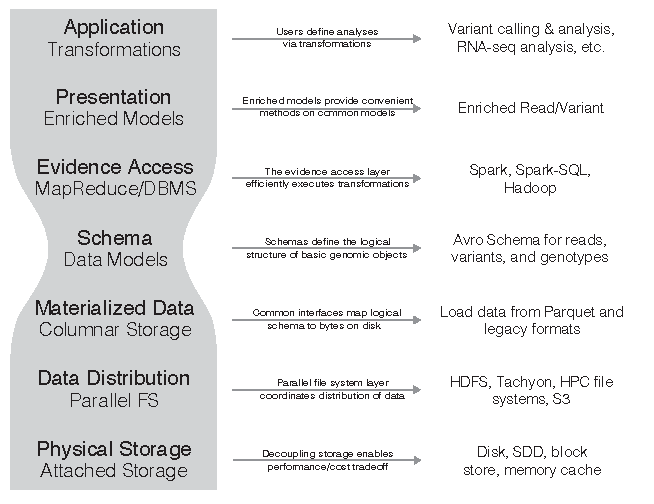
\includegraphics{graphs/expanded-stack-2.pdf}
\end{center}
\caption{A stack model for scientific computing}
\label{fig:stack-model}
\end{figure}

Unlike conventional scientific systems that leverage custom data formats like BAM or SAM~\cite{li09},
or CRAM~\cite{fritz11}, we believe that the use of an explicit schema for data interchange is critical.
In our stack model shown in Figure~\ref{fig:stack-model}, the schema becomes the ``narrow waist''
of the stack. Most importantly, placing the schema as the narrow waist enforces a strict separation
between data storage/access and data processing. Additionally, this enables literate programming
techniques which can clarify the data model and access patterns. The seven layers of our stack model
are decomposed as follows, and are numbered in ascending order from bottom to top:

\begin{enumerate}
\item \textbf{Physical Storage:} This layer coordinates data writes to physical media.
\item \textbf{Data Distribution:} This layer manages access, replication, and distribution of the files that have
been written to storage media.
\item \textbf{Materialized Data:} This layer encodes the patterns for how data is encoded and stored. This
layer determines I/O bandwidth and compression.
\item \textbf{Data Schema:} This layer specifies the representation of data, and forms the narrow waist of
the stack that separates access from execution.
\item \textbf{Evidence Access:} This layer provides us with primitives for processing data, and allows us to
transform data into different views and traversals.
\item \textbf{Presentation:} This layer enhances the data schema with convenience methods for performing
common tasks and accessing common derived fields from a single element.
\item \textbf{Application:} At this level, we can use our evidence access and presentation layers to compose
the algorithms to perform our desired analysis.
\end{enumerate}

A well defined software stack has several other significant advantages. By limiting application
interactions with layers lower than the presentation layer, application developers are given a clear and
consistent view of the data they are processing, and this view of the data is independent of whether the
data is local or distributed across a cluster or cloud. By separating the API from the data access layer,
we improve flexibility. With careful design in the data format and data access layers, we can seamlessly
support conventional whole file access patterns, while also allowing easy access to small slices of files.
By treating the compute substrate and storage as separate layers, we also drastically increase
the portability of the APIs that we implement.

As we discuss in more detail in~\S\ref{sec:read-preprocessing}, current scientific systems bleed
functionality between stack layers. An exemplar is the SAM/BAM and CRAM formats, which expect data
to be sorted by genomic coordinate. This order modifies the layout of data on disk~(level 3, Materialized Data)
and constrains how applications traverse datasets~(level 5, Evidence Access). Beyond
constraining applications, this leads to bugs in applications that are difficult to detect.
These views of evidence should be implemented at the evidence
access layer instead of in the layout of data on disk. This split enforces independence of anything below the
schema.

The idea of decomposing scientific applications into a stack model is not new; Bafna et al~\cite{bafna13}
made a similar suggestion in 2013. We borrow some vocabulary from Bafna et al, but our approach is
differentiated in several critical ways:

\begin{itemize}
\item Bafna et al consider the stack model specifically in the context of data management systems for
genomics; as a result, they bake current technologies and design patterns into the stack. In our opinion,
a stack design should serve to abstract layers from methodologies/implementations. If not, future
technology trends may obsolete a layer of the stack and render the stack irrelevant.
\item Bafna et al define a binary data format as the narrow waist in their stack, instead of a schema.
While these two seem interchangeable, they are not in practice. A schema is a higher level of abstraction
that encourages the use of literate programming techniques and allows for data serialization techniques
to be changed as long as the same schema is still provided.
\item Notably, Bafna et al use this stack model to motivate GQL~\cite{kozanitis14}. While a query system
should provide a way to process and transform data, Bafna et al instead move this system down to the
data materialization layer. We feel that this inverts the semantics that a user of the system would prefer
and makes the system less general.
\end{itemize}

Deep stacks like the OSI stack~\cite{zimmermann80} are generally simplified for practical use. Conceptually,
the stack we propose is no exception. In practice, we combine layers one and two, and layers five and six.
There are several reasons for these mergers. First, in \textsc{Hadoop}-based systems, the system does not have practical visibility
below layer two, thus there is no reason to split layers one and two except as a philosophical exercise.
Layers five and six are commingled because some of the enriched presentation objects are used to
implement functionality in the evidence access layer. This normally happens when a key is needed, such as
when repartitioning the dataset, or when reducing or grouping values.

\chapter{The \textsc{ADAM} Architecture}
\label{chap:architecture}

\textsc{ADAM}'s architecture was introduced as a response to the challenges
processing the growing volume of genomic sequencing data in a reasonable
timeframe~\cite{schadt10, stein10}. While the per-run latency of current genomic
pipelines such as the \textsc{GATK} could be improved by manually partitioning
the input dataset and distributing work, native support for distributed
computing is not provided. As a stopgap solution, projects like
\textsc{Cloudburst}~\cite{schatz09} and \textsc{Crossbow}~\cite{langmead09}
have ported individual analytics tools to run on top of \textsc{Hadoop}. While
this approach has served well for proofs of concept, this approach provides poor
abstractions for application developers. These poor abstractions make it
difficult for bioinformatics developers to create novel distributed genomic
analyses, and does little to attack sources of inefficiency or incorrectness in
distributed genomics pipelines.

\textsc{ADAM}'s architecture reconsiders how we build software for processing
genomic data by eliminating the monolithic architectures that are driven by the
underlying flat file formats used in genomics. These architectures impose
significant restrictions, including:

\begin{itemize}
\item These implementations are locked to a single node processing model. Even
  the \textsc{GATK}'s ``map-reduce'' styled \textsc{walker} API~\cite{mckenna10}
  is limited to natively support processing on a single node. While these jobs
  can be manually partitioned and run in a distributed setting, manual
  partitioning can lead to imbalance in work distribution and makes it difficult
  to run algorithms that require aggregating data across all partitions, and
  lacks the fault tolerance provided by modern distributed systems such as
  \textsc{Apache Hadoop} or \textsc{Spark}~\cite{zaharia12}.
\item Most of these implementations \emph{assume} invariants about the sorted
  order of records on disk. This ``stack smashing'' (specifically, the layout
  of data is used to ``accelerate'' a processing stage) can lead to bugs when
  data does not cleanly map to the assumed sort order. Additionally, since these
  sort order invariants are rarely explicit and vary from tool to tool,
  pipelines assembled from disparate tools can be brittle. We discuss this more
  in Chapter~\ref{chap:adam}.
\item Additionally, while these invariants are intended to improve performance,
  they do this at the cost of opacity. If we can express the query patterns that
  are accelerated by these invariants at a higher level, then we can achieve
  both a better programming environment and enable various query optimizations.
\end{itemize}

At the core of \textsc{ADAM}, users use the \textsc{ADAMContext} to load data as
\textsc{GenomicRDD}s, which they can then manipulate. Figure~\ref{fig:grdd}
depicts the \textsc{GenomicRDD} class hierarchy. In this class hierarchy, we
provide several classes that contain functionality that is applicable to all
genomic datatypes, such as the coordinate-space primitives described
in~\S\ref{sec:query-patterns} and the \textsc{pipe} primitive described
in~\S\ref{sec:pipe-api}, and the genomic metadata management described
in~\S\ref{sec:metadata}.

\begin{figure}[h]
\begin{center}
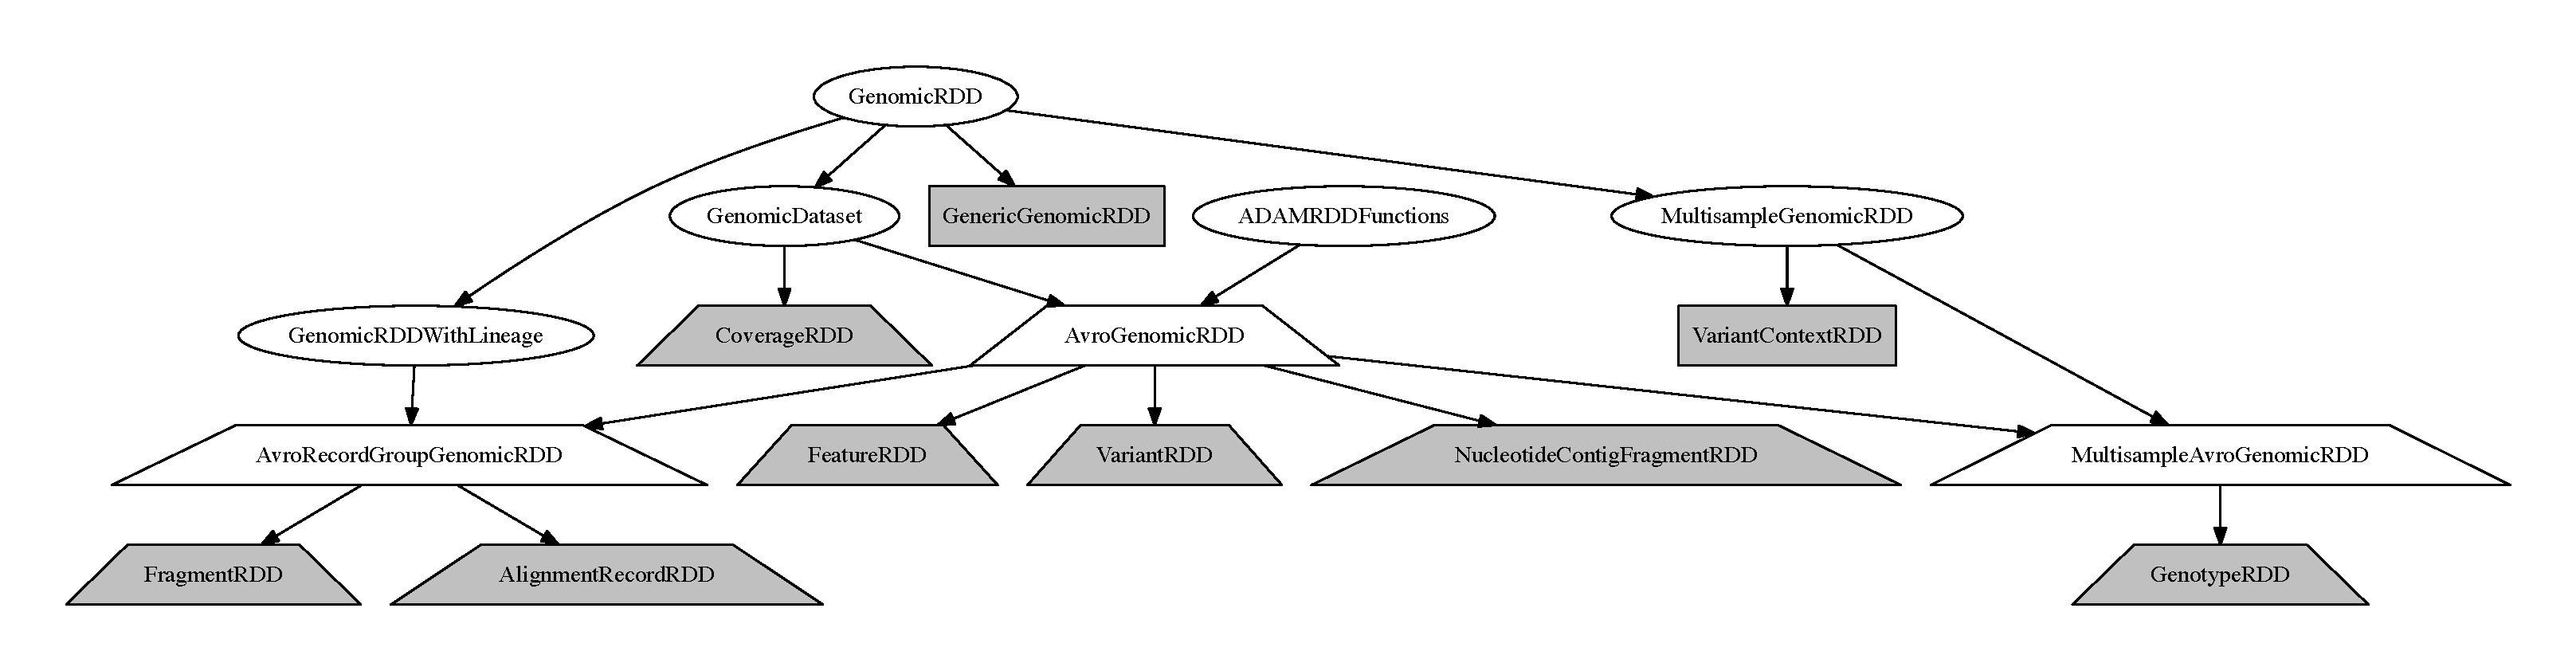
\includegraphics[width=0.95\linewidth]{graphs/grdd.pdf}
\end{center}
\caption{The \textsc{GenomicRDD} class hierarchy. Ovals are traits, trapezoids
  are abstract classes, rectangles are classes, and a bold border means that the
  abstract class is sealed. In \textsc{Scala}, sealing a class/trait restricts
  which classes can extend this class/mix-in this trait. The shaded classes are
  the types returned from the \textsc{ADAMContext} load methods and from the
  \textsc{GenomicRDD} methods.}
\label{fig:grdd}
\end{figure}

While the \textsc{ADAMContext} API has existed since the beginning of the
\textsc{ADAM} project, the \textsc{GenomicRDD} API is a fairly recent
introduction, having been added in 2016, three years into the project. Despite
its recent addition, the \textsc{GenomicRDD} API has been critical to achieving
the vision behind \textsc{ADAM}:

\begin{itemize}
\item The \textsc{GenomicRDD} wraps the \textsc{Apache Spark}
  RDD~\cite{zaharia12} and \textsc{Spark SQL} DataFrame~\cite{armbrust15} APIs
  with genomics-specific and genomic-datatype specific functionality. This
  enables the use of both generic~(RDD/DataFrame) and specialized APIs~(the
  region join and \textsc{pipe} APIs) to process genomic data in a natively
  distributed manner.
\item The rich \textsc{GenomicRDD} type hierarchy enables methodical management
  of genomics metadata. We support metadata management at a read group, sample,
  and computational lineage level.
\item By building upon APIs from \textsc{Spark SQL}, the \textsc{GenomicRDD} API
  can be exposed in the \textsc{Python} and R languages, which enables the use
  of \textsc{ADAM} outside of the JVM.
\end{itemize}

In the rest of this chapter, we explain the design decisions behind the
\textsc{ADAM} architecture, with an eye towards how the architecture has
evolved over the four years of the project. We discuss the specific tradeoffs
we needed to make in order to realize the stack architecture we had introduced,
before diving into the schema design that we used to decouple \textsc{ADAM} from
the genomics file formats. We review the genomics-specific query patterns
supported in \textsc{ADAM}, and explain how we have broadened \textsc{ADAM}'s
APIs to support multiple languages.

\section{Realizing A Decoupled Stack Architecture In \textsc{ADAM}}
\label{sec:realizing-stack-architecture}

While a stack-based architecture provides many of the benefits we asserted in
the previous section, these benefits can only be realized with careful API
design. If the APIs are specified at too low of a level of abstraction, then the
implementations of each layer will leak through, and the stack layers cannot be
exchanged. If the APIs are specified at too high of a level of abstraction, then
programmers who are implementing their applications on top of the APIs cannot
meaningfully reason about the performance and semantics of the code that they
are running.

In \textsc{ADAM}, we ultimately extend two important APIs. The
\textsc{ADAMContext} is the entrypoint to loading all data, while the
\textsc{GenomicRDD} API provides an abstract wrapper for genomic datasets. We
specialize the \textsc{GenomicRDD} API across the various genomic datatypes.
Once data has been loaded using the \textsc{ADAMContext}, users largely interact
with the data by transforming the data enclosed in a \textsc{GenomicRDD}, which
is described by our schemas~(see~\S\ref{sec:schema-design}). These core APIs
contribute to realizing the stack vision in the following ways:

\begin{itemize}
\item The physical storage and data distribution layers~(1 and 2) are largely
  deferred to \textsc{Apache Spark} and \textsc{Hadoop}. \textsc{ADAM} interacts
  with these layers through their APIs. There are a few places where
  \textsc{ADAM} specializes for a given file system; the primary example is when
  concatenating output files together to create a large unified output file. The
  \textsc{Hadoop Distributed File System}~(HDFS, see Shvachko et
  al.~\cite{shvachko10}) and the Amazon Web Services \textsc{Simple Storage
    System}~(AWS S3) provide APIs for concatenating sharded files, which allows
  the file merging process to be accelerated.
\item The materialized data and schema layers~(3 and 4) couple together in a
  critical way. The schemas provide a logical description of a given genomic
  datatype, and the materialized data layer provides a set of views between the
  \textsc{ADAM} schemas and legacy genomics file formats. This view is applied
  by the \textsc{ADAMContext} when loading data, and by the \textsc{GenomicRDD}
  when saving data. This decomposition is critically important: a common early
  misunderstanding of \textsc{ADAM} was that our schemas were introducing a new
  file format for genomic data. Rather, by supporting views between common
  formats to our schemas, we eliminate the need to know which file formats the
  data was loaded from.
\item The evidence access layer~(5) is largely implemented in the
  \textsc{GenomicRDD}, but can also be specialized in downstream applications
  for their specific application/query pattern. At a basic level, \textsc{ADAM}
  uses \textsc{Apache Spark}~\cite{zaharia12} and \textsc{Spark
    SQL}~\cite{armbrust15} for evidence access. Without any optimizations,
  queries are implemented as scans over the full dataset. However, we apply
  several optimizations for coordinate-based queries, as described
  in~\S\ref{sec:query-patterns}. Additionally, since \textsc{ADAM} builds off of
  \textsc{Spark}'s RDD API, any tools that optimize at the RDD level can be used
  to enrich the evidence access layer~\cite{tu16, morrow17}.
\item The presentation layer~(6) provides datatype~(e.g., read/feature/variant)
  specific methods on top of the \textsc{GenomicRDD} API. This includes
  many of the operations introduced in Chapter~\ref{chap:adam}.
\item The application layer~(7) is where the user builds their code, and this is
  built by using the \textsc{ADAMContext} to load in a \textsc{GenomicRDD},
  which is then transformed and saved.
\end{itemize}

While many of these layers have been unchanged since we introduced our stack
model in our original technical report~\cite{massie13} and our SIGMOD
manuscript~\cite{nothaft15}, the evidence access and presentation layers~(5 and
6) have changed. While the \textsc{ADAMContext} API has existed in \textsc{ADAM}
since the beginning of the project, the \textsc{GenomicRDD} API was only
introduced in 2016, three years into the project. The introduction of the
\textsc{GenomicRDD} API was symbolic of larger changes, which included:

\begin{itemize}
\item The evidence access layer originally assumed that other query systems like
  \textsc{Cloudera Impala}~\cite{kornacker15} would be able to interoperate with
  the \textsc{ADAM} schemas to load data. While this is still true, we have
  deemphasized this view. Specifically, once data has been loaded using the
  \textsc{ADAM} schemas and saved into \textsc{Apache Parquet}, systems like
  \textsc{Impala} can interoperate with the data through the \textsc{ADAM}
  schemas. However, systems like \textsc{Impala} cannot interoperate with
  the lower levels of \textsc{ADAM}'s stack, such as \textsc{ADAM}'s views to
  and from legacy genomics file formats.
\item Because the \textsc{Hadoop} ecosystem optimizes for full scans, we
  originally assumed that all queries were executed as full scans over the
  dataset, and these queries were executed without assuming any knowledge of the
  layout of the data. One of the advantages of introducing the
  \textsc{GenomicRDD} API is that we were better able to track the layout of
  data, and to specialize queries given a known layout. We describe one such
  mechanism for accelerating queries in the genomic coordinate space
  in~\S\textsc{sec:query-patterns}.
\item The presentation layer~(6) was originally implemented by enhancing the
  schemas. Specifically, the \textsc{AlignmentRecord}
  schema~(see~\S\ref{sec:read-schemas}) was accompanied by a
  \textsc{RichAlignmentRecord} class, which provided convenience methods on top
  of the schema. Similar ``enriched'' classes existed for the \textsc{Variant}
  schema as well. While these enriched classes have not been eliminated from
  \textsc{ADAM}, we have eliminated the public API exposure of these classes.
  While these classes were useful for implementing some of the algorithms in the
  \textsc{ADAM} core, they ultimately proved difficult to understand the
  performance characteristics of. They leveraged the \textsc{Scala} language's
  compile-time implicit conversion functionality~\cite{odersky04}, which allows for
  the compile-time inclusion of a method that can satisfy a given type
  signature. Additionally, the enriched classes typically augmented the raw
  schemas by lazily computing expensive values, which could then be reused
  across calculations. Unfortunately, the way these patterns intersected made it
  very difficult to reason about when a state had been calculated, and thus what
  the performance of a call to an enriched class would be. Additionally, the
  implicit conversion pattern could not be supported across languages, and was
  out of the scope of experise of the average bioinformatics programmer.
  Instead, we surfaced transformations at the dataset level, which is closer to
  the level of abstraction expected by our average user.
\end{itemize}

While the introduction of the \textsc{GenomicRDD} class has enabled the changes
to our stack model that were described above, it was driven by other factors.
The \textsc{ADAMContext} would originally return unwrapped \textsc{Spark} RDDs.
The introduction of the \textsc{GenomicRDD} class was driven largely by the need
for better management of genomic metadata, as described in~\S\ref{sec:metadata}.

\section{Schema Design for Representing Genomic Data}
\label{sec:schema-design}

A common criticism of bioinformatics as a field surrounds the proliferation of file formats. Short read data alone is
stored in four common formats: \textsc{FASTQ}~\cite{cock10}, \textsc{SAM}~\cite{li09}, \textsc{BAM}, and
\textsc{CRAM}~\cite{fritz11}. While these formats all represent different layouts of data on disk, they tend to be
logically harmonious. Due to this logical congruency of the different formats, we chose to build \textsc{ADAM}
on top of a logical schema, instead of a binary format on disk. While we do use Apache \textsc{Parquet}~\cite{parquet} to
materialize data on disk, the Apache \textsc{Avro}~\cite{avro} schema is used as a narrow waist in the system,
that enables ``legacy'' formats to be processed identically to data stored in \textsc{Parquet} with modest performance
degradation.

We made several high level choices when designing the schemas used in
\textsc{ADAM}~\cite{massie13}. Over time, we have gone backwards on some of
these design decisions. First, the schemas were originally fully denormalized.
Our rationale for thie decision was that this would reduce the cost of metadata
access while simplifying metadata distribution. We believed we would be able to
gain these benefits without greatly increasing the cost of memory access because
our backing store~(\textsc{Parquet}) made use of run length and dictionary
encoding, which allows for a single object to be allocated for highly repetitive
elements on read. As we discuss in~\S\ref{sec:metadata}, this decision wound up
being costly, and we reversed this decision as the \textsc{ADAM} schemas
progressed. Another key design choice was to require that all fields in the
schema are nullable; by enforcing this requirement, we enable arbitrary user
specified projections. Arbitrary projections can be used to accelerate
common sequence quality control algorithms such as Flagstat~\cite{massie13,
  nothaft15}. We have still maintained this requirement.

\begin{figure}[h]
\begin{center}
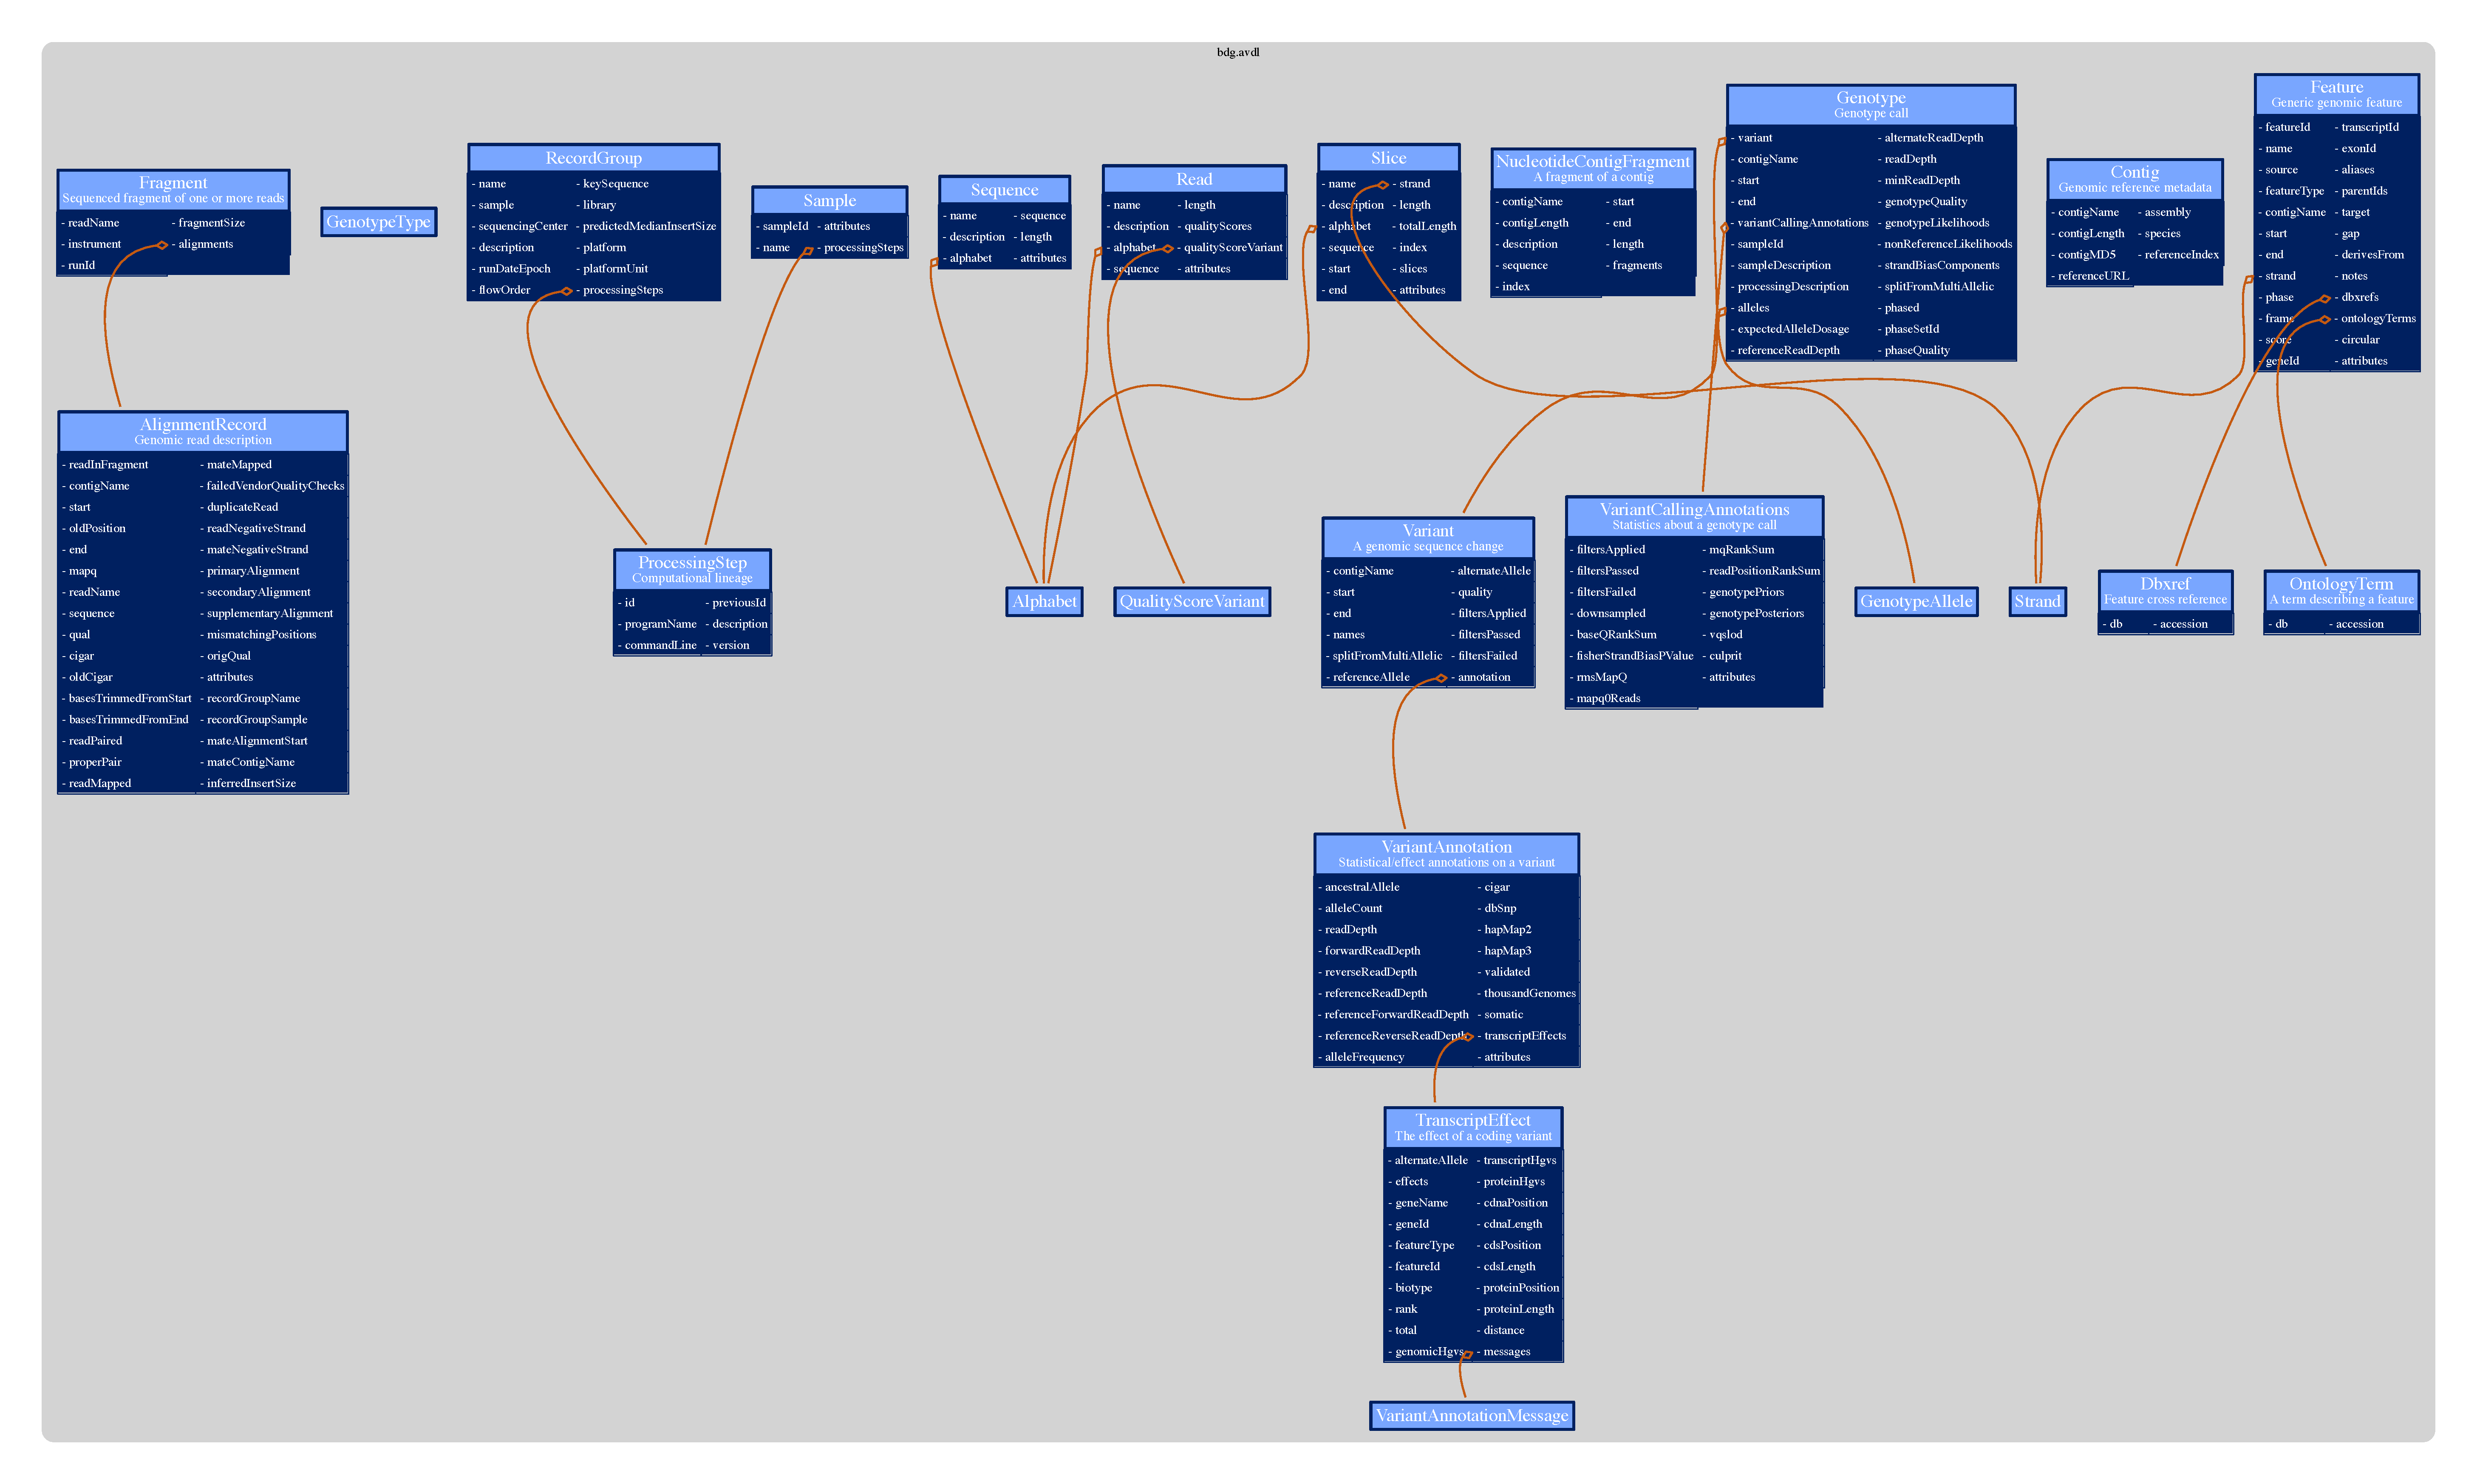
\includegraphics[width=0.95\linewidth]{graphs/bdg.pdf}
\end{center}
\caption{A UML diagram showing the dependencies and structure of the ADAM
  schemas. ADAM's read schema is fairly flat, which contrasts with the other
  schemas which employ nesting. The variant and feature schemas are deeply
  nested. This allows both rich annotation and the definition of the complex
  feature hierarchies necessary for describing genomic
  annotations~\cite{eilbeck05}.}
\label{fig:schemas}
\end{figure}

We have reproduced the schemas used to describe reads, features, variants, and
genotypes below. Figure~\ref{fig:schemas} is a UML diagram depicting how the
schemas connect. \textsc{ADAM} also contains schemas for describing assembled
contigs, but we have not included them in this section. We discuss the current
schemas, as well as their evolution over the course of the \textsc{ADAM}
project. While \textsc{ADAM}'s read schemas closely represent the \textsc{SAM}
specification, the variation and feature representations deviate significantly
from the current state of representing genomic variation and features.

\subsection{Read Schemas}
\label{sec:read-schemas}

Our read schema maps closely to the logical layout of data presented by
\textsc{SAM} and \textsc{BAM}. Unlike the \textsc{SAM} format, we split the
flags out from a single field into many fields. This makes it much simpler to
extract state from a record. Additionally, we promote several commonly used
fields from \textsc{SAM} attributes to fields. These fields include the original
quality, position, and CIGAR fields, which are set during
realignment~(see~\S\ref{sec:indel-realignment-implementation}) and base quality
recalibration~(see~\S\ref{sec:bqsr-implementation}).

\begin{lstlisting}[caption=\textsc{ADAM} read schema]
record AlignmentRecord {
 
  union { int, null } readInFragment = 0;

  union { null, string } contigName = null;
  union { null, long } start = null;
  union { null, long } oldPosition = null;
  union { null, long } end = null;

  union { null, int } mapq = null;

  union { null, string } readName = null;

  union { null, string } sequence = null;
  union { null, string } qual = null;

  union { null, string } cigar = null;
  union { null, string } oldCigar = null;

  union { int, null } basesTrimmedFromStart = 0;
  union { int, null } basesTrimmedFromEnd = 0;

  union { boolean, null } readPaired = false;
  union { boolean, null } properPair = false;
  union { boolean, null } readMapped = false;
  union { boolean, null } mateMapped = false;
  union { boolean, null } failedVendorQualityChecks = false;
  union { boolean, null } duplicateRead = false;

  union { boolean, null } readNegativeStrand = false;
  union { boolean, null } mateNegativeStrand = false;
  union { boolean, null } primaryAlignment = false;
  union { boolean, null } secondaryAlignment = false;
  union { boolean, null } supplementaryAlignment = false;

  union { null, string } mismatchingPositions = null;
  union { null, string } origQual = null;

  union { null, string } attributes = null;

  union { null, string } recordGroupName = null;
  union { null, string } recordGroupSample = null;

  union { null, long } mateAlignmentStart = null;
  union { null, string } mateContigName = null;

  union { null, long } inferredInsertSize = null;
}
\end{lstlisting}

Additionally, we support a schema that groups together all of the reads from a
single sequenced fragment. This fragment enables a traversal over read data that
is similar to \textsc{SAM}'s read-name grouping.

\begin{lstlisting}[caption=\textsc{ADAM} fragment schema]
record Fragment {

  union { null, string } readName = null;

  union { null, string } instrument = null;
  union { null, string } runId = null;

  union { null, int } fragmentSize = null;

  array<AlignmentRecord> alignments = [];
}
\end{lstlisting}

We feel that the fragment schema is preferable to the queryname sort order and
query grouping invariants that \textsc{SAM} allows one to specify. By using this
schema, we can reduce the cost of duplicate marking by
50\%~(see~\S\ref{sec:benchmarking-duplicate-markers}). Additionally, this
representation provides a useful alternative to the interleaved FASTQ format for
streaming reads into an aligner. We demonstrate this usage in
Chapter~\ref{chap:cannoli}.

\subsection{Variation Schemas}
\label{sec:variation-schemas}

The variant and genotype schemas present a larger departure from the representation used by the Variant Call
Format~(\textsc{VCF}). The most noticeable difference is that we have migrated away from \textsc{VCF}'s variant oriented
representation to a matrix representation. Instead of the variant record serving to group together genotypes, the
variant record is embedded within the genotype. Thus, a record represents the genotype assigned to a sample,
as opposed to a \textsc{VCF} row, where all individuals are collected together. The second major modification is to assume
a biallelic representation. In a biallelic representation, we describe the genotype of a sample at a position or
interval as the composition of a reference allele and a single alternate allele. If multiple alternate alleles segregate at
the site (e.g., there are two known SNPs in a population at this site), we create multiple biallelic variants for the site.
This differs from \textsc{VCF}, which allows multiallelic records. By limiting
ourselves to a biallelic representation, we are able to clarify the meaning of many of the variant calling annotations. If a
site contains a multiallelic variant (e.g., in \textsc{VCF} parlance this could be a \textsc{1/2} genotype), we split the
variant into two or more biallelic records. The sufficient statistics for each allele should then be computed under
a reference model similar to the model used in genome \textsc{VCF}s. If the sample does contain a multiallelic variant at
the given site, this multiallelic variant is represented by referencing to another record via the \textsc{OtherAlt}
enumeration. A similar biallelic model is also used by the \textsc{Hail} project~\cite{hail}.

\begin{lstlisting}[caption=\textsc{ADAM} core variant and genotype schemas]
record Variant {

  union { null, string } contigName = null;
  union { null, long } start = null;
  union { null, long } end = null;

  array<string> names = [];

  union { boolean, null } splitFromMultiAllelic = false;

  union { null, string } referenceAllele = null;
  union { null, string } alternateAllele = null;

  union { null, double } quality = null;

  union { null, boolean } filtersApplied = null;
  union { null, boolean } filtersPassed = null;
  array<string> filtersFailed = [];

  union { null, VariantAnnotation } annotation = null;
}

enum GenotypeAllele {
  REF,
  ALT,
  OTHER_ALT,
  NO_CALL
}

record Genotype {

  union { null, Variant } variant = null;
  union { null, string } contigName = null;
  union { null, long } start = null;
  union { null, long } end = null;

  union { null, VariantCallingAnnotations } variantCallingAnnotations = null;

  union { null, string }  sampleId = null;
  union { null, string }  sampleDescription = null;
  union { null, string }  processingDescription = null;

  array<GenotypeAllele> alleles = [];

  union { null, float } expectedAlleleDosage = null;
  union { null, int } referenceReadDepth = null;
  union { null, int } alternateReadDepth = null;
  union { null, int } readDepth = null;
  union { null, int } minReadDepth = null;

  union { null, int } genotypeQuality = null;
  array<double> genotypeLikelihoods = [];
  array<double> nonReferenceLikelihoods = [];

  array<int> strandBiasComponents = [];

  union { boolean, null } splitFromMultiAllelic = false;

  union { boolean, null } phased = false;
  union { null, int } phaseSetId = null;
  union { null, int } phaseQuality = null;
}
\end{lstlisting}

The variant and genotype schemas are the schemas that have evolved the most
over the course of the \textsc{ADAM} project. When we wrote the original
\textsc{ADAM} technical report~\cite{massie13}, the variant and genotype schemas
were much narrower and closely mirrored the \textsc{VCF} specification.
Since the VCF format contains many attributes that can be used to annotate both
a genotype~(via a \textsc{Format} field) or a variant~(via an \textsc{Info}
field), the original schemas largely contained overlapping field definitions.
We refactored the two schemas to move to the biallelic-only variant model, and
later, expanded the variant schema to include a nested structural variant
description. This structural variant schema was removed during a large refactor
after the ADAM SIGMOD paper that improved support for variant annotations. We
have also played with flattening the variant schema out of the genotype schema
for performance reasons. During our work on \textsc{Mango}~cite{tu16, morrow17},
we realized that nesting the variant field decreased the performance of range
queries by approximately an order of magnitude. In the variant annotation
refactor, we added the schemas below.

\begin{lstlisting}[caption=\textsc{ADAM} variant annotation schemas]
record TranscriptEffect {
  union { null, string } alternateAllele = null;

  array<string> effects = [];

  union { null, string } geneName = null;
  union { null, string } geneId = null;
  union { null, string } featureType = null;
  union { null, string } featureId = null;
  union { null, string } biotype = null;

  union { null, int } rank = null;
  union { null, int } total = null;

  union { null, string } genomicHgvs = null;
  union { null, string } transcriptHgvs = null;
  union { null, string } proteinHgvs = null;

  union { null, int } cdnaPosition = null;
  union { null, int } cdnaLength = null;

  union { null, int } cdsPosition = null;
  union { null, int } cdsLength = null;

  union { null, int } proteinPosition = null;
  union { null, int } proteinLength = null;

  union { null, int } distance = null;

  array<VariantAnnotationMessage> messages = [];
}

record VariantAnnotation {

  union { null, string } ancestralAllele = null;

  union { null, int } alleleCount = null;

  union { null, int } readDepth = null;
  union { null, int } forwardReadDepth = null;
  union { null, int } reverseReadDepth = null;
  union { null, int } referenceReadDepth = null;
  union { null, int } referenceForwardReadDepth = null;
  union { null, int } referenceReverseReadDepth = null;

  union { null, float } alleleFrequency = null;

  union { null, string } cigar = null;

  union { null, boolean } dbSnp = null;
  union { null, boolean } hapMap2 = null;
  union { null, boolean } hapMap3 = null;
  union { null, boolean } validated = null;
  union { null, boolean } thousandGenomes = null;

  union { boolean, null } somatic = false;

  array<TranscriptEffect> transcriptEffects = [];

  map<string> attributes = {};
}
\end{lstlisting}

These schemas provide a faithful representation of the VCF/ANN specification,
which adds a formal and rich variant annotation specification to
VCF~\cite{ann}. This specification is used by both the \textsc{Ensembl Variant
  Effect Predictor}~(VEP, see~\cite{mclaren10}) and \textsc{SnpEff}~\cite{cingolani12}.
We have a separate schema for storing annotations on top of a genotype call; we
refer to this object as a ``variant calling annotation'' instead of a ``genotype
annotation,'' since the annotations are specific to the variant calling process
and the reads observed at the site, as opposed to the called genotype.

\begin{lstlisting}[caption=\textsc{ADAM} genotype annotation schema]
record VariantCallingAnnotations {

  union { null, boolean } filtersApplied = null;
  union { null, boolean } filtersPassed = null;
  array<string> filtersFailed = [];

  union { null, boolean } downsampled = null;

  union { null, float } baseQRankSum = null;
  union { null, float } fisherStrandBiasPValue = null;
  union { null, float } rmsMapQ = null;
  union { null, int } mapq0Reads = null;
  union { null, float } mqRankSum = null;
  union { null, float } readPositionRankSum = null;

  array<float> genotypePriors = [];
  array<float> genotypePosteriors = [];

  union { null, float } vqslod = null;
  union { null, string } culprit = null;

  map<string> attributes = {};
}
\end{lstlisting}

The variant calling annotations object includes annotations that we feel are
useful during the variant calling process, but that should probably be omitted
from a final callset that is used for annotation and statistical testing. Many
of these variant annotations are useful for hard filtering, as described
in~\S\ref{sec:variant-filtration}.

During the refactor that improved \textsc{ADAM}'s support for variant
annotations, we refactored the conversion class that provided a view from the
VCF format to \textsc{ADAM}'s genotype and variant records. In this refactor,
we replaced the extant conversion code with a pure-functional converter. Our
approach generated a collection of conversion functions. To convert between
the \textsc{ADAM} and \textsc{htsjdk} representations of a variant/genotype,
we would fold over this collection of functions. In turn, each function accesses
the field they are converting, and mutates the new object that is being built
during the conversion. The use of a pure-functional converter had several
upsides:

\begin{itemize}
\item One of the difficulties in working with the VCF file format is that it is
  semi-structured and user extensible. Beyond the info and format attributes
  in the VCF specification, users can add any attributes they desire, restricted
  only by the attribute types in the VCF specification. As part of this update,
  we added the ability to generate attribute conversion functions from the VCF
  header.
\item Our new converter has a single function per field that is converted. As a
  result, it is very easy to write highly directed functional tests to achieve a
  very high level of test coverage for the converter. Since the functions are
  all orthogonal and have no shared state, we can also guarantee that any two
  functions that independently pass their directed tests can be called in a
  chain correctly.
\item A minor problem with our previous, monolithic converters was that they
  could not support projecting out a subset of fields, unlike data stored in
  \textsc{Apache Parquet} using the \textsc{ADAM} schemas. While we would
  still need to read all of the data in a whole row, being able to limit the
  number of fields projected would reduce the amount of parsing we need to do,
  which can be quite costly for semi-structured text formats like VCF. The
  pure-functional converter naturally supports user-specified projections, as we
  can arbitrarily filter out any conversion functions that we do not want to
  execute.
\end{itemize}

In the long term, we hope to apply this pure-functional conversion approach to
all of our data converters. We discuss this more in~\S\ref{sec:lazy-bind}.

\subsection{Feature Schemas}
\label{sec:feature-schemas}

\textsc{ADAM}'s feature schema provides an abstracted view of a genomic feature
that can support most of the various genomic feature file formats, including
\textsc{NarrowPeak}, BED, GTF/GFF2, GFF3, and \textsc{IntervalList}. We have
full support for nested features, which are commonly used for describing genome
annotations. Instead of nesting the features recursively inside of the feature
record, we leverage the database cross reference schema, which is derived from
the GTF/GFF2/GFF3 file format.

\begin{lstlisting}[caption=\textsc{ADAM}'s feature schemas]
enum Strand {
  FORWARD,
  REVERSE,
  INDEPENDENT,
  UNKNOWN
}

record Dbxref {
  union { null, string } db = null;
  union { null, string } accession = null;
}

record OntologyTerm {
  union { null, string } db = null;
  union { null, string } accession = null;
}

record Feature {

  union { null, string } featureId = null;
  union { null, string } name = null;

  union { null, string } source = null;

  union { null, string } featureType = null;

  union { null, string } contigName = null;
  union { null, long } start = null;
  union { null, long } end = null;

  union { null, Strand } strand = null;

  union { null, int } phase = null;
  union { null, int } frame = null;

  union { null, double } score = null;

  union { null, string } geneId = null;
  union { null, string } transcriptId = null;
  union { null, string } exonId = null;
  array<string> aliases = [];
  array<string> parentIds = [];

  union { null, string } target = null;

  union { null, string } gap = null;

  union { null, string } derivesFrom = null;

  array<string> notes = [];

  array<Dbxref> dbxrefs = [];

  array<OntologyTerm> ontologyTerms = [];

  union { null, boolean } circular = null;

  map<string> attributes = {};
}
\end{lstlisting}

\textsc{ADAM} originally contained an additional \textsc{GenomeRDD} subclass
called the \textsc{GeneRDD}. This class would take the nested features contained
in a \textsc{FeatureRDD} that described an annotated genome, and would perform
all the joins and aggregations necessary to build out the fully nested
annotation structure. Ultimately, we removed this class because the performance
was poor, and most queries that would run on the nested structure could be
refactored to run on the flattened feature hierarchy. This was possible due to
the denormalized schema, which included the transcript and gene IDs in each
feature record.

\subsection{Managing Genomic Metadata}
\label{sec:metadata}

A major evolution of the \textsc{ADAM} schemas relates to how we manage and
store metadata. In our original schemas, the metdata was denormalized across the
record. For example, all of the metadata from the sequencing run and prior
processing steps were packed into record group metadata fields, as opposed to
being stored in a file header. Our rationale was that this metadata describes
the processing lineage of the sample and is expected to have limited cardinality
across all records, and thus would compresses extremely well.

This metadata is string heavy, and benefitted strongly from column-oriented
decompression on disk. However, proper deserialization from disk proved to be
difficult. Although the information consumes less than 5\% of space on disk, a
poor deserializer implementation may replicate a string per field per record,
which greatly increased the amount of memory allocated and the garbage
collection~(GC) load. With this metadata included in each record, a dataset
that was 200GB on disk would balloon into more than 5TB in memory. Additionally,
implementing the deserializer conflicted with \textsc{Apache Spark}'s
serialization architecture. \textsc{Spark} assumes that deserializers have
limited state, and write to a stream that does not support seeks. While this is
a reasonable assertion for row-oriented serialization techinques, this made it
extremely difficult to implement a column-oriented serialization. Prior to
eliminating the denormalized metadata from our schemas, this meant that we would
have very efficient memory utilization immediately after reading from disk, as
\textsc{Apache Parquet} would only allocate a single string per replicated
element. However, we would then see the memory explosion after the first shuffle
in our query.

This memory explosion led to a major refactor of the \textsc{ADAM} schemas and
the introduction of the \textsc{GenomicRDD} hierarchy. Originally, since the
metadata was consolidated in each record, the \textsc{ADAMContext} load methods
would return \textsc{RDD}s containing our \textsc{Apache Avro}~\cite{avro}
schema objects. The methods that made up the presentation layer~(6) of our stack
would be added at compile-time using \textsc{Scala}'s implicit methods. When we
refactored the schemas, we introduced the \textsc{GenomicRDD} classes as a way
to track metadata alongside the \textsc{Apache Spark} RDD, moved the
presentation layer methods into the implementations of the \textsc{GenomicRDD}
classes, and eliminated the implicit conversions. Long term, we believe that the
ideal mechanism for storing this metadata is a database designed for storing
metadata, such as the \textsc{Ground} store~\cite{hellerstein17}. We discuss the
longterm metadata managment needs in~\S\ref{sec:metadata-future}.

\section{Query Patterns for Genomic Data Analysis}
\label{sec:query-patterns}

There are a wide array of experimental techniques and platforms in genome
informatics, but many of these methods produce datapoints that are tied to
locations in the genome through the use of genomic coordinates. A platform
for scientific data processing in genomics needs to understand these
1-dimensional coordinate systems because these become the basis on which
data processing is parallelized. For example, when calling variants from
sequencing data, the sequence data that is localized to a single genomic
locus can be processed independently from the data localized to a different
region.

Beyond parallelization, many of the core algorithms and methods for data
aggregation in genomics are phrased in terms of geometric primitives on 1-D
intervals and points where we compute distance, overlap, and containment. An
algorithm for calculating quality control metrics may try to calculate coverage,
a count of how many reads overlap each base in the genome. A method for
filtering and annotating potential variants might assess the validity of a
variant using the quality characteristics of all reads that overlap the
putative variant.

To support these algorithms, we provide the region join primitive. The algorithm
used is described in algorithm~\ref{alg:region-join} and takes as input two RDDs
of \textsc{ReferenceRegions}, a data structure that represents intervals along
the 1-D genomics coordinate space. It produces the set of all overlapping
\textsc{ReferenceRegion} pairs. This join can be implemented using either a
broadcast or sort-merge approach. Algorithm~\ref{alg:region-join} demonstrates
the broadcast approach.

\begin{algorithm}
\caption{Join Regions via Broadcast}
\label{alg:region-join}
\begin{algorithmic}
\STATE $left \leftarrow$ input dataset; left side of join
\STATE $right \leftarrow$ input dataset; right side of join
\STATE $sortedLeft \leftarrow left$.sort()
\STATE $collectedLeft \leftarrow sortedLeft$.collect()
\STATE $tree \leftarrow collectedLeft$.buildTree()
\STATE $broadcastTree \leftarrow tree$.broadcast()
\STATE $joined \leftarrow right$.map($r \rightarrow broadcastTree$.overlaps($r$))
\RETURN $joined$
\end{algorithmic}
\end{algorithm}

Our implementation of the broadcast region join has been refactored twice. The
first implementation was described in our SIGMOD manuscript~\cite{nothaft15} and
required the computation of the convex hulls of the left side of the dataset.
This was done using an algorithm similar to the one described
in~\S\ref{sec:convex-hull}. Additionally, this approach required both sides to
be hash-partitioned. The first rewrite of the broadcast join was very similar to
Algorithm~\ref{alg:region-join}. However, it used an interval
tree~\cite{samet90} to store the left side of the join. We abandoned this
approach because of the cost of serializing the interval tree. Instead, we
introduced a new data structure, the interval array, which is a flattened
representation of the interval tree. The interval array is an array whose
elements are sorted by coordinate-order. To look up overlapping elements from an
interval array, we begin by running binary search to find the first element that
overlaps our search value. In the interval array, we also compute and store the
length of the longest region in the array. We then search forward in the array
until we have searched the distance of the longest element. Since this data
structure is flat, it is inexpensive to (de)serialize. Binary search provides
the same $\mathcal{O}(\log n)$ time complexity as searching into an interval
tree. However, since we require an additional linear search, we can only
guarantee the best case $\Theta(\log n)$ complexity for searching into our
interval array.

While the join described above is a broadcast join, a region join can also be
implemented via a straightforward shuffle-based approach, which is described in
Algorithm~\ref{alg:shuffle-region-join}. The \textsc{partitionJoinFn} function
maintains two iterators (one each from both the left and right collections),
along with a buffer. This buffer is used to track all key-value pairs from the
right collection iterator that \emph{could} match to a future key-value pair
from the left collection iterator. We prune this buffer every time that we
advance the left collection iterator. For simplicity, the description of
Algorithm~\ref{alg:shuffle-region-join} ignores the complexity of processing
keys that cross partition boundaries. In our implementation, we replicate keys
that cross partition boundaries into both partitions.

\begin{algorithm}
\caption{Partition And Join Regions via Shuffle}
\label{alg:shuffle-region-join}
\begin{algorithmic}
\STATE $left \leftarrow$ input dataset; left side of join
\STATE $right \leftarrow$ input dataset; right side of join
\STATE $partitions \leftarrow left$.getPartitions()
\STATE $left \leftarrow left$.repartitionAndSort($partitions$)
\STATE $right \leftarrow right$.repartitionAndSort($partitions$)
\STATE $joined \leftarrow left$.zipPartitions($right$, \textsc{partitionJoinFn})
\RETURN $joined$
\end{algorithmic}
\end{algorithm}

These joins serve as a core that we can use to build other abstractions with.
For example, self-region joins and multi-region joins are common in genomics,
and can be easily implemented using the above implementations. We are currently
working to implement further parallel spatial functions such as sliding windows,
using techniques similar to the shuffle-based join. Additionally, we are working
to improve the performance of these joins by eliminating shuffles of data that
is already sorted on disk. We discuss these avenues for future work
in~\S\ref{sec:extensions-adam}.

\section{Supporting Multi-Language Processing in \textsc{ADAM}}
\label{sec:multi-language}

One of the original goals in using \textsc{Apache Avro} was to allow the
\textsc{ADAM} schemas to be used across more languages than just \textsc{Scala}
and \textsc{Java}, as \textsc{Avro} has language bindings for commonly used
languages like C/C++/C\#, \textsc{Python}, and \textsc{JavaScript}. However,
this wound up not being a fruitful exercise. While \textsc{Avro} supported these
languages, \textsc{Apache Parquet} did not, and since we used \textsc{Avro} to
manage in-memory serialization but \textsc{Parquet} to manage on-disk
serialization, users could not load our \textsc{Parquet} files from disk in
non-JVM languages. Additionally, even if we had support for reading
\textsc{Parquet} files from these other languages, it would've been prohibitive
to port all of the logic in our stack~(mostly at the materialized data and
presentation layers) over to other languages.

Instead, we followed the approach used by \textsc{Apache Spark}'s
\textsc{Python} and R bindings~\cite{venkataraman16} after \textsc{Spark SQL}
was introduced~\cite{armbrust15}. Here, we created lightweight wrappers for
the \textsc{ADAMContext} and \textsc{GenomicRDD} in the \textsc{Python} and
R languages. These wrappers then called the JVM implementations of these classes
through \textsc{Py4j}~\cite{py4j} or \textsc{SparkR}'s interoperability
layer~\cite{venkataraman16}. Instead of exposing the underlying RDD, we exposed
the parallel dataset through \textsc{Spark SQL}'s \textsc{DataFrame} API. We
chose this for several reasons:

\begin{itemize}
\item The \textsc{DataFrame} API is a close match to the programming models
  commonly used in \textsc{Python} and R~\cite{armbrust15}, such as the
  \textsc{Pandas}~\cite{mckinney10} and \textsc{Dyplr}~\cite{wickham15} libraries.
\item A major performance pitfall in \textsc{PySpark} and \textsc{SparkR} was
  serializer performance. Specifically, to use \textsc{PySpark}, we would have
  needed to transform our binary \textsc{Avro} records into textual records that
  \textsc{PySpark} would pickle for use in \textsc{Python}.
\item Additionally, the \textsc{Spark SQL} query engine~\cite{armbrust15} allows
  \textsc{Python} and R users to write query plans that can then be optimized
  and executed using optimized JVM implementations where possible. This is a
  contrast to \textsc{Spark}'s RDD API, where both records and queries are black
  boxes.
\end{itemize}

While building on \textsc{Spark SQL} enabled cross-language support, it was not
a straightforward process. Specifically, \textsc{Spark SQL} leveraged several
\textsc{Scala} language features that were incompatible with our \textsc{Avro}
schema representation. To address this, we built automation that translates
between \textsc{Spark SQL}'s desired representation and \textsc{Avro} at compile
time.

\begin{figure}[h]
\begin{center}
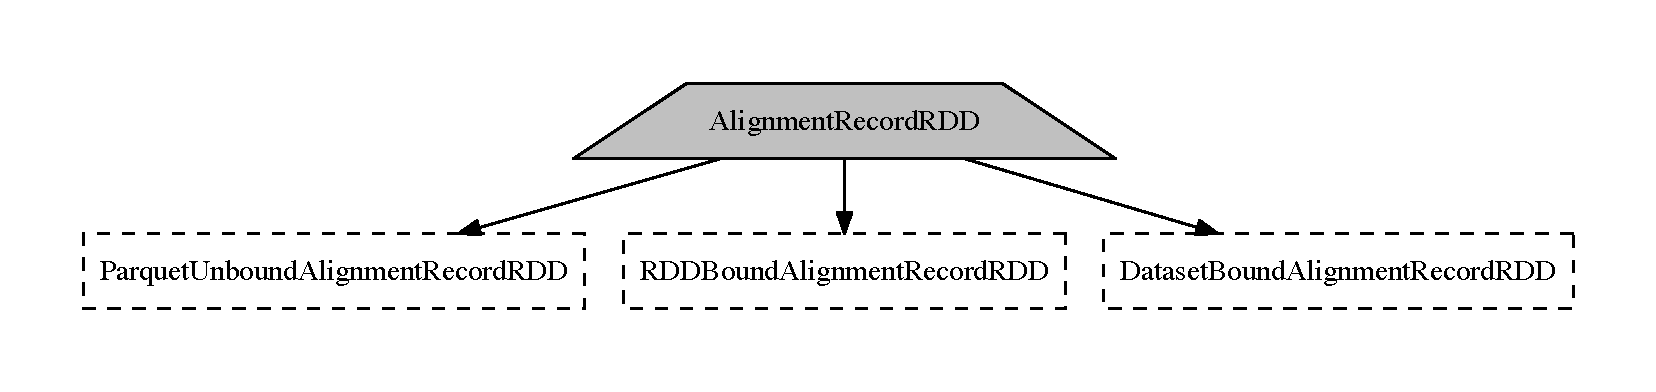
\includegraphics[width=0.5\linewidth]{graphs/binding.pdf}
\end{center}
\caption{With the move to support \textsc{Spark SQL}, we added a binding scheme
  to the \textsc{GenomicRDD} hierarchy. This figure depicts the alternative
  bindings available for the \textsc{AlignmentRecordRDD}, which is
  representative of the core \textsc{GenomicRDD} types. The dotted lines around
  the concrete implementations of the abstract \textsc{AlignmentRecordRDD} class
  signify that these classes are protected and cannot be instantiated outside of
  the \textsc{ADAM} library.}
\label{fig:binding}
\end{figure}

Since translating between a \textsc{Spark} RDD and a \textsc{Spark SQL}
DataFrame requires a (de)serialization pass, we introduced a scheme that we call
``lazy binding'' to minimize serialization overhead. In Figure~\ref{fig:grdd},
you may have noticed that most of the core \textsc{GenomicRDD} types were
sealed abstract classes. In practice, they are all implemented using the lazy
binding scheme. Figure~\ref{fig:binding} depicts the bound variants of the
\textsc{AlignmentRecordRDD} type. In this scheme, we track whether the last
transformation applied to the \textsc{GenomicRDD} was applied to the DataFrame
or RDD representation of the genomic data. The next phase of computation will
run on top of the bound output of the prior stage. This can provide a major
performance win if running \textsc{Spark SQL} queries, as the \textsc{Spark SQL}
query optimizer performs major optimizations to amortize the method call
overhead of chained transformations~\cite{armbrust15}. A further optimization
deals with loading data from \textsc{Apache Parquet}. While data that is being
loaded from legacy file formats like BAM or VCF must be loaded as an RDD,
\textsc{Parquet} can be loaded as either an RDD or DataFrame, and \textsc{Spark
  SQL} can make further optimizations if it knows that it is loading data from
\textsc{Parquet}. To handle this, we added the ``unbound'' \textsc{GenomicRDD}.
This datatype does not bind to the RDD or DataFrame representation of a
\textsc{Parquet} table until a transformation is invoked. We believe that there
are further opportunities to extend lazy binding to legacy genomic file formats,
which we discuss in~\S\ref{sec:lazy-bind}.

\part{Algorithms and Tools}

\chapter{Automatic Parallelization of Legacy Tools with \textsc{Cannoli}}
\label{chap:cannoli}

While \textsc{ADAM} provides a general API for implementing genomic analyses
using \textsc{Apache Spark}, we will never be able to fully eliminate single
node tools from genomic workflows. Beyond the small set of tools discussed
in~\S\ref{sec:distributed-genome-analysis}, the majority of genomics tools are
designed to run on a single node. Additionally, due to memory access and
allocation patterns, tools like aligners pay a steep performance penalty when
moving out of C/C++ to the JVM. An example of this is the \textsc{SNAP} aligner,
which was originally written on \textsc{Apache Spark}, before being rewritten in
C++ for performance~\cite{zaharia11}. Finally, while it is possible to
reimplement common genomic analyses like variant calling using \textsc{ADAM}, it
is not feasible to do this across the hundreds of extant genomic analyses.

As discussed in~\S\ref{sec:distributed-genome-analysis}, there are many tools
that provide customized solutions to this problem. The GATK's \textsc{Queue}
engine~\cite{depristo11} could be used to run the GATK in parallel, and the
\textsc{FreeBayes} variant caller~\cite{garrison12} can be run in parallel
through the \textsc{SpeedSeq} pipeline~\cite{chiang15}. Additionally, a variety
of tools are parallelized by \textsc{Hadoop}-ecosystem wrappers. These include
tools like the \textsc{Seal} tool which parallelizes \textsc{BWA} using
\textsc{Pydoop}~\cite{leo10, pireddu11}, \textsc{Rail-RNA}~\cite{nellore16},
which was built on top of \textsc{Hadoop}, and tools built on top of
\textsc{Hadoop Streaming} like \textsc{CrossBow}~\cite{langmead09crossbow} for
SNP calling and \textsc{Cloudburst}~\cite{schatz09} for alignment.
Additionally, several tools have built on top of \textsc{Apache Spark},
including \textsc{CloudScale-BWAMEM}~\cite{chen16} and
\textsc{BWASpark}~\cite{abuin16}.

Instead of expecting developers to create a proliferation of custom wrappers for
parallelizing tools on distributed analysis systems, we should be able to build
a general infrastructure to automatic this process. Since many genomics tools
are built around a streaming paradigm, if we can provide automated chunking,
process setup, distribution of reference files, and streaming data, we should
be able to automatically parallelize a large number of genomic analysis tools.

In this chapter, we introduce a two part architecture for automatically
parallelizing genomic analyis tools. First, we describe ADAM's \textsc{pipe}
API, which performs the automated chunking, resource distribution, and process
coordination. Then, we describe the \textsc{Cannoli} tool, which contains
wrappers for a set of common genomic analysis tools. This approach is general
but not universal: while the \textsc{pipe} API can be used to parallelize the
majority of analysis steps, it cannot be used for tools that require an
all-reduce. This includes RNA-seq quantification tools like
\textsc{Kallisto}~\cite{bray16} or \textsc{Salmon}~\cite{patro17}, or tools
that perform a global normalization, like the XHMM copy number variant
caller~\cite{fromer12}. However, this approach works well for tools whose
computation can be described as mapping over unaligned reads, or mapping over
data aligned to a genomic locus range.

\section{Accomodating Single-node Tools in \textsc{ADAM} With the \textsc{pipe} API}
\label{sec:pipe-api}

The \textsc{pipe} API is an API in \textsc{ADAM} that provides a simple
mechanism for automatically parallelizing a command across a cluster running
\textsc{Apache Spark}. The user specifies the command to be run, files that need
to be distributed to each worker running the command, and any environment
settings that are needed. \textsc{ADAM} then uses the attached genomic reference
metadata~(see~\S\ref{sec:metadata}) to infer the proper partitioning to apply to
the data, partitions the data, and runs the user specified command. The input
format to provide to the command and the output format to expect from the
command is determined at compile-time in \textsc{Scala} and at runtime in R and
\textsc{Python}.

\begin{figure}[h]
\begin{center}
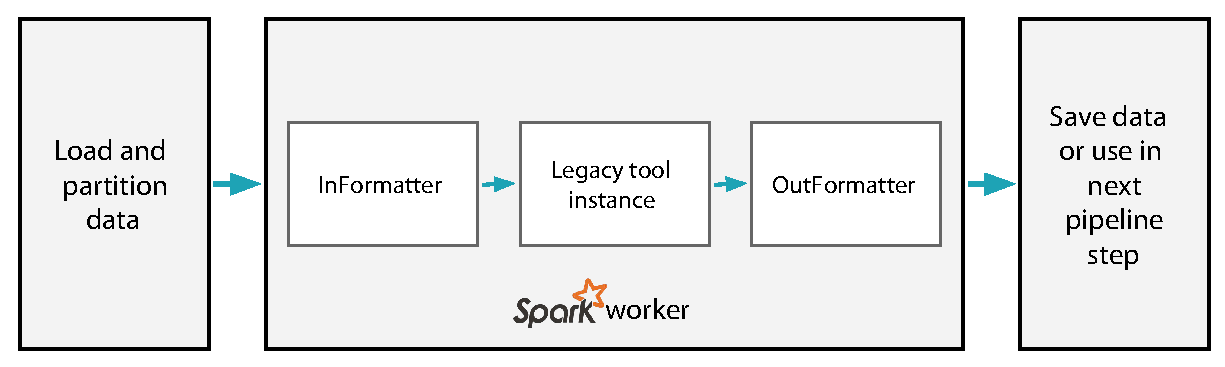
\includegraphics[width=0.95\linewidth]{graphs/pipe.pdf}
\end{center}
\caption{The implementation of the \textsc{pipe} API.}
\label{fig:pipe}
\end{figure}

Figure~\ref{fig:pipe} illustrates how the \textsc{pipe} API is executed by
\textsc{ADAM}. The \textsc{pipe} implementation starts by checking the genome
reference metadata~(see~\S\ref{sec:metadata}) to see if the dataset is aligned
to a reference genome. If the data is not aligned, then we assume that no
specific partitioning scheme is needed, and skip repartitioning. If the data is
aligned, then we use the partitioner used in the region join
implementation~(see~\S\ref{sec:query-patterns}) to chunk the data into
partitions that represent contiguous blocks of the reference genome. After the
partitioning phase, we open a subprocess per partition that is running the user
specified command, and connect streams to the standard in and out pipes of the
running process.

To handle a wide variety of file formats, we have abstracted the I/O subsystem
into ``formatters.'' We use the formatters to encode/decode the data going to
and from the running process:

\begin{itemize}
\item To create the input for the running process, we use the
  \textsc{InFormatter} trait. This trait receives an iterator over a single
  partition of a \textsc{GenomicRDD}, and encodes that iterator into the format
  that the running process is expecting. Each implementation of the
  \textsc{InFormatter} trait is required to also implement the
  \textsc{InFormatterCompanion} trait, which defines a singleton object that
  can create an instance of the class. This pattern is necessary to expose
  the metadata stored in a \textsc{GenomicRDD} to the \textsc{InFormatter} by
  guaranting that there will be a static method that can build an
  \textsc{InFormatter} with access to the metadata stored in a
  \textsc{GenomicRDD}. This approach is necessary since \textsc{Scala} cannot
  guarantee that each implementation of a trait provides a constructor with a
  given type signature, and we need metadata to construct properly formatted
  BAM and VCF streams. The \textsc{InFormatter} runs asynchronously in a new
  thread.
\item To read the data from the running process, we use the
  \textsc{OutFormatter} trait. This trait decodes the output of an invocation of
  the running process and creates an iterator. The \textsc{OutFormatter} does
  not need access to the metadata from a \textsc{GenomicRDD}, so we do not need
  an \textsc{OutFormatterCompanion} trait. The \textsc{OutFormatter} is run
  synchronously in the thread that called the process. The \textsc{OutFormatter}
  provides an iterator so that we can leverage \textsc{Apache Spark}'s pulling
  model, which limits the number of records that must be materialized into
  memory at a given instant.
\end{itemize}

This API allows for a very concise, yet general framework. With the
formatter pattern, we can support a broad range of formats while exposing a
very simple API to the user. Specifically, we can pipe sequence fragments as
interleaved FASTQ, reads as SAM/BAM/CRAM, variants/genotypes as VCF, and
features as BED/GTF/GFF2/GFF3/\-\textsc{IntervalList}/\-\textsc{NarrowPeak}. If
a program needs reference files to be available locally on each node, they can
achieve this by passing an array containing the URLs of each file. We use an
internal \textsc{Apache Spark} API to copy these files locally on each machine.
Along with this, we provide a simple syntax that allows the user to symbolically
add the local path to this file into their command, which we know at runtime.

To demonstrate how concise the API is, Listings~\ref{lst:pipe-bwa}
and~\ref{lst:pipe-freebayes} demonstrate how to use the \textsc{pipe}
API to call BWA~\cite{li09bwa} from \textsc{Python} and
\textsc{FreeBayes}~\cite{garrison12} from R.

\begin{lstlisting}[caption=Calling BWA using the \textsc{Python pipe} API, label=lst:pipe-bwa]
from bdgenomics.adam.adamContext import ADAMContext

ac = ADAMContext(sc)

reads = ac.loadAlignments("reads.fastq").toFragments()

alignedReads = reads.pipe(
  "bwa mem -t 1 -p /data/hs38DH.fa -",
  "org.bdgenomics.adam.fragments.InterleavedFASTQInFormatter",
  "org.bdgenomics.adam.rdd.read.AnySAMOutFormatter",
  "org.bdgenomics.adam.api.java.FragmentsToAlignmentRecordsConverter")
\end{lstlisting}

\begin{lstlisting}[caption=Calling \textsc{FreeBayes} using the R \textsc{pipe} API, label=lst:pipe-freebayes]
library(bdg.adam)

ac <- ADAMContext(sparkR.session())

reads <- loadAlignments(ac, "alignments.bam")

variants <- pipe(reads,
  "freebayes --fasta-reference /data/hs38DH.fa --stdin",
  "org.bdgenomics.adam.rdd.read.BAMInFormatter",
  "org.bdgenomics.adam.rdd.variant.VCFOutFormatter",
  "org.bdgenomics.adam.api.AlignmentRecordsToVariantContextsConverter")
\end{lstlisting}

In both examples, the user can run the parallelized tool with less than five
lines of code. We believe that the power of this API lies in its simplicity.
With a minimal API, we can replace the manual sharding that was historically
implemented using workflow management systems~\cite{depristo11, chiang15} or
custom wrappers~\cite{langmead09, schatz09, pireddu11, nellore16}. Since this
API is built in the query layer of the \textsc{ADAM} stack, it can run
independent of both the file format used to save the data and the storage
system used to store the data. This latter point is a significant improvement
over workflow systems that expect a shared POSIX file system, as these systems
often use indexed range query into a file to perform sharding~\cite{chiang15}.
This is difficult to apply generally on a cloud file store like S3, as then the
tool being run in parallel must be able to natively query the cloud file system.
Additionally, this approach makes it possible to integrate a command line
program into a larger programmatic workflow. We discuss a possible use case that
would leverage this pattern in~\S\ref{sec:efficient-consensus}.

\section{Packaging Parallelized Single-node Tools in \textsc{Cannoli}}
\label{sec:parallelizing-in-cannoli}

To make the automated parallelization of the \textsc{pipe} API more accessible
to users, we introduced the \textsc{Cannoli} tool, which provides a command line
interface~(CLI) for executing common tools using the \textsc{pipe} API. Our
goals were to provide a minimal wrapper around the \textsc{pipe} API that would:

\begin{itemize}
\item Allow the user to use reference files that were already present locally on
  all nodes in the cluster, or automatically distribute the necessary reference
  files to all nodes.
\item Support running the tool from a locally installed executable or a
  \textsc{Docker} container, as \textsc{Docker} is becoming a widely used method
  for distributing pre-built genomic analysis tools~\cite{vivian17}.
\end{itemize}

To support this, we have control logic that parses out the arguments passed to
the CLI. If the user has requested that we distribute all of the files to the
workers, we then elaborate out the paths needed by the tool and add the files
to the \textsc{pipe} call. We do this since many tools that require prebuilt
resources use a multitude of resource files that are all at a base path. For
example, BWA~\cite{li09bwa} uses seven index files, SNAP~\cite{zaharia11} uses
four index files, and \textsc{SnpEff}~\cite{cingolani12} uses a large directory of
resource files. If the user has requested to run the tool via a \textsc{Docker}
container, we then ensure that the directory containing the distributed
index files are accessible within the container. Currently, we support a list of
tools including but not limited to BWA, SNAP, and
\textsc{Bowtie2}~\cite{langmead09bowtie} for alignment;
\textsc{FreeBayes}~\cite{garrison12} and \textsc{mpileup}~\cite{li11} for
variant calling; and \textsc{SnpEff} and \textsc{BEDTools}~\cite{quinlan10} for
annotation. We evaluate the performance and concordance of the tools implemented
in \textsc{Cannoli} in~\S\ref{sec:benchmarking-cannoli}.

\chapter{Scalable Alignment Preprocessing with \textsc{ADAM}}
\label{chap:adam}

In \textsc{ADAM}, we have implemented the three most commonly used pre-processing stages from the
\textsc{GATK} pipeline~\cite{depristo11}. In this section, we describe the stages that we have
implemented, and the techniques we have used to improve performance and accuracy when running on
a distributed system. These pre-processing stages include:

\begin{enumerate}
\item Duplicate marking: During the process of preparing DNA for sequencing, reads are duplicated by
errors during the sample preparation and polymerase chain reaction stages. Detection of duplicate reads
requires matching all reads by their position and orientation after read alignment. Reads with identical position
and orientation are assumed to be duplicates. When a group of duplicate reads is found, each read is scored,
and all but the highest quality read are marked as duplicates.

We have validated our duplicate removal code against Picard~\cite{picard}, which is used by the GATK
for Marking Duplicates. Our implementation is fully concordant with the Picard/GATK duplicate removal
engine, except we are able to perform duplicate marking for read pairs whose reads align to different
reference chromosomes~(known as chimeric read pairs, see Li et al~\cite{li10}).
Specifically, because Picard's traversal engine is restricted to processing linearly sorted alignments,
Picard mishandles these alignments. Since our engine is not constrained by the underlying layout of data
on disk, we are able to properly handle chimeric read pairs.
\item Local realignment: In local realignment, we correct areas where variant alleles cause reads to be
locally misaligned from the reference genome. This is typically caused by the presence of
insertion/deletion (INDEL) variants~\cite{depristo11}. In this algorithm, we first identify regions
as targets for realignment. In the \textsc{GATK}, this identification is done by traversing sorted read alignments. In our implementation,
we fold over partitions where we generate targets, and then we merge the tree of targets. This process allows us
to eliminate the data shuffle needed to achieve the sorted ordering. As part of this fold, we must
compute the convex hull of overlapping regions in parallel. We discuss this in more detail later in this section.

After we have generated the targets, we associate reads to the overlapping target, if one exists. After
associating reads to realignment targets, we run a heuristic realignment algorithm that works by minimizing
the quality-score weighted number of bases that mismatch against the reference.
\item Base Quality Score Recalibration: During the sequencing process, systemic errors occur
that lead to the incorrect assignment of base quality scores. In this step, we label each base that we have
sequenced with an error covariate. For each covariate, we count the total number of bases that we saw,
as well as the total number of bases within the covariate that do not match the reference genome. From this data, 
we apply a correction by estimating the error probability for each set of covariates under a beta-binomial model
with uniform prior.

We have validated the concordance of our BQSR implementation against the GATK. Across both tools, only 5000
of the $\sim$180B bases~($<0.0001\%$) in the high-coverage NA12878 genome dataset differ. After investigating
this discrepancy, we have determined that this is due to an error in the GATK, where paired-end reads are
mishandled if the two reads in the pair overlap.
\end{enumerate}

In the rest of this section, we discuss the high level implementations of these algorithms.
We evaluate the performance and concordance of these algorithms against other
tools in~\S\ref{sec:benchmarking-preprocessing}.

\section{BQSR Implementation}
\label{sec:bqsr-implementation}

Base quality score recalibration seeks to identify and correct correlated errors in base quality score estimates.
At a high level, this is done by associating sequenced bases with possible error covariates, and estimating the
true error rate of this covariate. Once the true error rate of all covariates has been estimated, we then apply
the corrected covariate.

The original BQSR engine in \textsc{ADAM} was written to be generic and to place
no limitations on the number or type of covariates that could be applied. A
covariate describes a parameter space where variation in the covariate parameter
may be correlated with a sequencing error. However, supporting generic covariates
reduced the throughput of the recalibration engine, and we found that
recalibration was generally run with two specified covariates. Currently, we
support two covariates that map to common sequencing errors~\cite{nakamura11}:

\begin{itemize}
\item \textsc{CycleCovariate}: This covariate expresses which cycle the base was
  sequenced in. Read errors are known to occur most frequently at the start or
  end of reads. Additionally, a reagent error can occur in a way that corrupts
  bases from a single cycle.
\item \textsc{DinucCovariate}: This covariate covers biases due to the sequence
  context surrounding a site. The two-mer ending at the sequenced base is used
  as the covariate parameter value.
\end{itemize}

These covariates are calculated for each sequenced base. We then merge the
covariates into a \textsc{CovariateKey}, which also includes the read group
that the sample was from~(see~\S\ref{sec:metadata}) and the quality score
assigned to the base. To generate the covariate observation table, we
aggregate together the number of observed and error bases per covariate.
Algorithms~\ref{alg:emit-observations} and \ref{alg:create-table} demonstrate
this process. In Algorithm~\ref{alg:emit-observations}, the \textsc{Observation}
class stores the number of bases seen and the number of errors seen. For
example, \textsc{Observation(1, 1)} creates an \textsc{Observation} object that
has seen one base, which was an erroneous base.

\begin{algorithm}
\caption{Emit Observed Covariates}
\label{alg:emit-observations}
\begin{algorithmic}
\STATE $read \leftarrow$ the read to observe
\STATE $covariates \leftarrow$ covariates to use for recalibration
\STATE $sites \leftarrow$ sites of known variation
\STATE $observations \leftarrow \emptyset$
\FOR{$base \in read$}
\STATE $covariate \leftarrow$ identifyCovariate($base$)
\IF{isUnknownSNP($base, sites$)}
\STATE $observation \leftarrow$ Observation($1, 1$)
\ELSE
\STATE $observation \leftarrow$ Observation($1, 0$)
\ENDIF
\STATE $observations$.append($(covariate, observation)$)
\ENDFOR
\RETURN $observations$
\end{algorithmic}
\end{algorithm}

\begin{algorithm}
\caption{Create Covariate Table}
\label{alg:create-table}
\begin{algorithmic}
\STATE $reads \leftarrow$ input dataset
\STATE $covariates \leftarrow$ covariates to use for recalibration
\STATE $sites \leftarrow$ known variant sites
\STATE $sites$.broadcast()
\STATE $observations \leftarrow reads$.map($read \Rightarrow$ emitObservations($read, covariates, sites$))
\STATE $table \leftarrow$ $observations$.reduceByKey(merge)
\RETURN $table$
\end{algorithmic}
\end{algorithm}

Originally, Algorithm~\ref{alg:create-table} was implemented by running an
aggregate where we merged all of the disparate covariates into the table at each
step. By restricting the BQSR engine to two covariates, we achieved several
performance optimizations:

\begin{itemize}
\item By hard-coding the types of covariates we used, we reduced the cost of
  identifying whether two \textsc{CovariateKey} objects represented the same
  covariate.
\item Additionally, hard-coding the covariates greatly reduced the size of the
  \textsc{CovariateKey} object in memory, which allows us to achieve higher
  cache hit rates when caching the output of the first stage of BQSR.
\item Merging the observations between two base observations originally required
  updating and merging the new and old \textsc{Observation} values. By rewriting
  as a \textsc{reduceByKey}, we were able to eliminate the need for mutable
  objects. We did not move this codepath to \textsc{Spark SQL}, since this
  refactor predated the introduction of \textsc{Spark SQL} support into ADAM.
  However, this is a straightforward modification.
\item In the process of rewriting the \textsc{CovariateKey} representation, we
  optimized the implementation of the code that assigned dinucleotide and cycle
  covariates to a given base. This yielded a $3\times$ speedup for the cycle
  covariate, and a $5\times$ speedup for the dinucleotide covariate.\cite{fixme}
\end{itemize}

Once we have computed the observations that correspond to each covariate, we
estimate the observed base quality using equation~\eqref{eqn:bqsr-err}. This
represents a Bayesian model of the mismatch probability with Binomial
likelihood and a Beta(1, 1) prior.

\begin{equation}
\label{eqn:bqsr-err}
\mathbf{E}(P_{err}|{cov}) = \frac{\textsc{\#errors}(cov) + 1}{\textsc{\#observations}(cov) + 2}
\end{equation}

After these probabilities are estimated, we go back across the input read
dataset and reconstruct the quality scores of the read by using the covariate
assigned to the read to look into the covariate table. However, this process is
expensive if implemented na\"{i}vely. To handle covariate specific errors, we
use the hierarchical model from the \textsc{GATK}~\cite{depristo11}. In this
model, we generate the empirical quality of a \textsc{CovariateKey} by
hierarchically computing the empirical error rates for the covariate
groups that it falls into. We treat the read group as the highest order
covariate, then the quality score, and then the two error covariates.
Algorithm~\ref{alg:invert-cov} demonstrates this approach.

\begin{algorithm}
\caption{Inverting an element in the covariate table}
\label{alg:create-table}
\begin{algorithmic}
\STATE $key \leftarrow$ covariate key to invert
\STATE $global \leftarrow$ the empirical quality of this read group
\STATE $qualities \leftarrow$ the empirical qualities of bases with a given quality score
\STATE $dinucs \leftarrow$ the empirical qualities of bases with a given context
\STATE $cycles \leftarrow$ the empirical qualities of bases at a given cycle
\STATE $p_1 \leftarrow$ compensate($key$.quality, $global$)
\STATE $p_2 \leftarrow$ compensate($p_1$, $qualities$($key$.quality)
\STATE $d_d \leftarrow$ delta($p_2$, $dinucs$($key$.dinuc))
\STATE $d_c \leftarrow$ delta($p_2$, $cycles$($key$.cycle))
\RETURN $p_2 + d_d + d_c$
\end{algorithmic}
\end{algorithm}

In the original BQSR implementation, this inversion would be called on every
read base. This is inefficient, as the empirical quality is equal across all
bases from a given \textsc{CovariateKey}. We eliminated this by inverting all
covariates after all of the observations had been collected. Then, evaluating
the new empirical quality score for a base assigned to a covariate was performed
by looking up the covariate key in a hash map, which is computationally
inexpensive.

\section{Indel Realignment Implementation}
\label{sec:indel-realignment-implementation}

Although global alignment will frequently succeed at aligning reads to the proper region of the genome, the local
alignment of the read may be incorrect. Specifically, the error models used by aligners may penalize local alignments
containing INDELs more than a local alignment that converts the alignment to a series of mismatches. To correct
for this, we perform local realignment of the reads against consensus sequences in a three step
process. In the first step, we identify candidate sites that have evidence of an insertion or deletion. We then compute
the convex hull of these candidate sites, to determine the windows we need to realign over. After these regions are
identified, we generate candidate haplotype sequences, and realign reads to minimize the overall quantity of mismatches
in the region.

\subsection{Realignment Target Identification}
\label{sec:realignment-target-identification}

To identify target regions for realignment, we simply map across all the reads. If a read contains INDEL evidence,
we then emit a region corresponding to the region covered by that read.

\subsubsection{Convex-Hull Finding}
\label{sec:convex-hull}

Once we have identified the target realignment regions, we must then find the maximal convex hulls
across the set of regions. For a set $R$ of regions, we define a maximal convex hull as the largest
region $\hat{r}$ that satisfies the following properties:

\begin{align}
\label{eqn:convexity-constraint}
\hat{r} &= \cup_{r_i \in \hat{R}} r_i \\
\hat{r} \cap r_i &\ne \emptyset, \forall r_i \in \hat{R} \\
\hat{R} &\subset R
\end{align}

In our problem, we seek to find all of the maximal convex hulls, given a set of regions. For genomics, the
convexity constraint described by equation \eqref{eqn:convexity-constraint} is trivial to check: specifically, the
genome is assembled out of reference contigs that define disparate 1-D coordinate spaces. If two regions exist on different contigs, they
are known not to overlap. If two regions are on a single contig, we simply check to see if they overlap
on that contig's 1-D coordinate plane.

Given this realization, we can define Algorithm~\ref{alg:parallel-convex-hull}, which is a data parallel
algorithm for finding the maximal convex hulls that describe a genomic dataset.

\begin{algorithm}
\caption{Find Convex Hulls in Parallel}
\label{alg:parallel-convex-hull}
\begin{algorithmic}
\STATE $data \leftarrow$ input dataset
\STATE $regions \leftarrow data$.map($data \Rightarrow $generateTarget($data$))
\STATE $regions \leftarrow regions$.sort()
\STATE $hulls \leftarrow regions$.fold($r_1, r_2 \Rightarrow$ mergeTargetSets($r_1, r_2$))
\RETURN $hulls$
\end{algorithmic}
\end{algorithm}

The \textsc{generateTarget} function projects each datapoint into a Red-Black tree that contains a
single region. The performance of the fold depends on the efficiency of the merge function. We achieve
efficient merges with the tail-call recursive \textsc{mergeTargetSets} function that is described in
Algorithm~\ref{alg:join-targets}.

\begin{algorithm}
\caption{Merge Hull Sets}
\label{alg:join-targets}
\begin{algorithmic}
\STATE $first \leftarrow$ first target set to merge
\STATE $second \leftarrow$ second target set to merge
\REQUIRE $first$ and $second$ are sorted
\IF{$first = \emptyset \wedge second = \emptyset$}
\RETURN $\emptyset$
\ELSIF{$first = \emptyset$}
\RETURN $second$
\ELSIF{$second = \emptyset$}
\RETURN $first$
\ELSE
\IF{last($first$) $\cap$ head($second$) $= \emptyset$}
\RETURN $first$ + $second$
\ELSE
\STATE $mergeItem \leftarrow$ (last($first$) $\cup$ head($second$))
\STATE $mergeSet \leftarrow$ allButLast($first$) $\cup mergeItem$
\STATE $trimSecond \leftarrow$ allButFirst($second$)
\RETURN mergeTargetSets($mergeSet$, $trimSecond$)
\ENDIF
\ENDIF
\end{algorithmic}
\end{algorithm}

The set returned by this function is used as an index for mapping reads directly to realignment targets.

\subsubsection{Candidate Generation and Realignment}
\label{sec:candidate-generation-realignment}

Once we have generated the target set, we map across all the reads and check to see if the read overlaps
a realignment target. We then group together all reads that map to a given realignment target; reads that
don't map to a target are randomly assigned to a ``null'' target. We do not attempt realignment for reads mapped
to null targets.

To process non-null targets, we must first generate candidate haplotypes to realign against. We support several
processes for generating these consensus sequences:

\begin{itemize}
\item \emph{Use known INDELs}: Here, we use known variants that were provided by the user to generate
consensus sequences. These are typically derived from a source of common variants such as dbSNP~\cite{sherry01}.
\item \emph{Generate consensuses from reads}: In this process, we take all INDELs that are contained in
the alignment of a read in this target region.
\item \emph{Generate consensuses using Smith-Waterman}: With this method, we take all reads that were
aligned in the region and perform an exact Smith-Waterman alignment~\cite{smith81} against the reference in this site. We
then take the INDELs that were observed in these realignments as possible consensuses. 
\end{itemize}

From these consensuses, we generate new haplotypes by inserting the INDEL consensus into the reference
sequence of the region. Per haplotype, we then take each read and compute the quality score weighted Hamming
edit distance of the read placed at each site in the consensus sequence. We then take the minimum quality
score weighted edit versus the consensus sequence and the reference genome. We aggregate these scores
together for all reads against this consensus sequence. Given a consensus sequence $c$, a reference sequence $R$,
and a set of reads $\mathbf{r}$, we calculate this score using equation~\eqref{eqn:realignment}.

\begin{align}
\label{eqn:realignment}
q_{i, j} &= \sum_{k = 0}^{l_{r_i}} Q_k I[r_I(k) = c(j + k)] \forall r_i \in \mathbf{R}, j \in \{0, \dots, l_c - l_{r_i}\}  \\
q_{i, R} &= \sum_{k = 0}^{l_{r_i}} Q_k I[r_I(k) = c(j + k)] \forall r_i \in \mathbf{R}, j = \text{pos}(r_i | R) \\
q_i &= \min(q_{i, R}, \min_{j \in \{0, \dots, l_c - l_{r_i}\}} q_{i, j}) \\
q_c &= \sum_{r_i \in \mathbf{r}} q_i
\end{align}

In~\eqref{eqn:realignment}, $s(i)$ denotes the base at position $i$ of sequence
$s$, and $l_s$ denotes the length of sequence $s$. We pick the consensus
sequence that minimizes the $q_c$ value. To improve performance, in the
$q_{i, j}$ calculation, we terminate the loop once the running sum
$\sum_{k = 0}^{l_{r_i}} Q_k I[r_I(k) = c(j + k)]$ is larger than the prior
$\min_i q_{i, j}$. If the chosen consensus has a log-odds ratio~(LOD)
that is greater than $5.0$ with respect to the reference, we realign the reads.
This is done by recomputing the CIGAR and MDTag for each new alignment.
Realigned reads have their mapping quality score increased by 10 in the Phred
scale.

\section{Duplicate Marking Implementation}
\label{sec:duplicate-marking-implementation}

Reads may be duplicated during sequencing, either due to clonal duplication via PCR before sequencing, or
due to optical duplication while on the sequencer. To identify duplicated reads, we apply a heuristic algorithm
that looks at read fragments that have a consistent mapping signature. First, we bucket together reads that
are from the same sequenced fragment by grouping reads together on the basis of read name and record group.
Per read bucket, we then identify the 5' mapping positions of the primarily aligned reads.
We mark as duplicates all read pairs that have the same pair alignment locations, and all unpaired reads that
map to the same sites. Only the highest scoring read/read pair is kept, where the score is the sum of all quality
scores in the read that are greater than 15.

To eliminate a shuffle, we leveraged an insight from
\textsc{SAMBLASTER}~\cite{faust14}, which runs directly on the output of an
aligner, which will group all reads from a single fragment together~(also known
as query grouped). The fragment schema introduced in~\S\ref{sec:read-schemas}
describes a set of query grouped reads, and is equivalent to the output of the
step in duplicate marking that groups reads by read name. This allows us to
eliminate a shuffle when running on reads loaded from a query grouped
SAM/BAM/CRAM file, or when running on the output of reads aligned using
\textsc{Cannoli}. We describe the performance benefit of this change
in~\S\ref{sec:benchmarking-duplicate-markers}.

\chapter{Rapid Variant Calling with \textsc{Avocado}}
\label{chap:avocado}

This chapter introduces \textsc{Avocado}, a substitution and short INDEL variant
caller that is built natively on top of the \textsc{ADAM} APIs. For highest
accuracy, \textsc{Avocado} is run as a two phase tool. In the first phase, we
reassemble or realign our reads around INDEL variants. In the second phase, we
apply a probabilistic model built around a biallelic model to the reads to
identify variants.

\textsc{Avocado}'s INDEL reassembly process cleans up all reads that are aligned
near INDEL variants. We do this as a two step process. In the first pass, we
pass over all the reads and use our novel indexed de Bruijn algorithm to extract
and canonicalize all of the INDEL variants. For best accuracy, we use the
\textsc{ADAM} INDEL realigner described
in~\S\ref{sec:indel-realignment-implementation} in knowns mode. This improves
variant calling accuracy over solely using the indexed de Bruijn algorithm.

After realigning the INDELs, we run genotyping. In this phase, we discover all
SNVs and INDELs, score them using the reads, and emit either called variants
or genotype likelihoods in genome VCF~(gVCF) format. This runs as a four step
process:

\begin{enumerate}
\item We extract all variants from the aligned reads by parsing the alignments.
\item Using these variants, we compute all read/variant overlaps, and compute
the likelihood that each read represents a given variant that it overlaps. In
gVCF mode, we also calculate the likelihood of the reference allele at all
locations covered by a read.
\item We merge all of the per-read likelihoods per variant. This gives us final
genotype likelihoods per each variant.
\item Finally, we apply a standard set of hard filters to each variant.
\end{enumerate}

All of these stages are implemented as a parallel application that runs on top of
\textsc{Apache Spark}~\cite{zaharia10, zaharia12}, using the \textsc{ADAM}
library~\cite{massie13, nothaft15}.

\section{INDEL Reassembly}
\label{sec:indel-reassembly}

As opposed to traditional realignment based approaches, we canonicalize INDELs
in the reads by looking for bubbles flanked by read vs. reference sequence matches. In a colored de Bruijn
graph, a bubble refers to a location where the graph diverges between two
samples. In \S\ref{sec:formulation}, we demonstrate how we can use the
reconvergence of the de Bruijn graph in the flanking sequence around a bubble
to define provably canonical alignments of the bubble between two sequences.
For a colored de Bruijn graph containing reads and the reference genome, this
allows us to canonically express INDEL variants in the reads against the
reference. In~\S\ref{sec:implementation}, we then show how this approach
can be implemented efficiently without building a de Bruijn graph per read,
or even adding each read to a de Bruijn graph. Once we have extracted a
canonical set of INDELs, we realign the reads to each INDEL sequence using
\textsc{ADAM}'s INDEL realigner, in known INDELs mode. For a full description
of the INDEL realignment process, see~\S\ref{sec:indel-realignment-implementation}.

\subsection{Preliminaries}
\label{sec:formulation}

Our method relies on an \emph{indexed de Bruijn} graph, which is a slight
extension of the colored de Bruijn graph~\cite{iqbal12}. Specifically, each
$k$-mer in an indexed de Bruijn graph knows which sequence position~(index)
it came from in its underlying read/sequence. To construct an indexed de
Bruijn graph, we start with the traditional formulation of a \emph{de Brujin}
graph for sequence assembly:

\begin{defn}[de Bruijn Graph]
\label{defn:dbg}
A de Bruijn graph describes the observed transitions between adjacent $k$-mers in a sequence. Each
$k$-mer $s$ represents a $k$-length string, with a $k - 1$ length prefix given by $\text{prefix}(s)$ and a
length 1 suffix given by $\text{suffix}(s)$. We place a directed edge ($\rightarrow$) from $k$-mer $s_1$ to
$k$-mer $s_2$ if $\text{prefix}(s_1)^{\{1, k - 2\}} + \text{suffix}(s_1) = \text{prefix}(s_2)$.
\end{defn}

Now, suppose we have $n$ sequences $\mathcal{S}_1, \dots, \mathcal{S}_n$. Let us assert that for each
$k$-mer $s \in \mathcal{S}_i$, then the output of function $\text{index}_i(s)$ is defined. This function
provides us with the integer position of $s$ in sequence $\mathcal{S}_i$. Further, given two $k$-mers
$s_1, s_2 \in \mathcal{S}_i$, we can define a distance function
$\text{distance}_i(s_1, s_2) = | \text{index}_i(s_1) - \text{index}_i(s_2) |$. To create an indexed
de Bruijn graph, we simply annotate each $k$-mer $s$ with the $\text{index}_i(s)$ value for all
$\mathcal{S}_i, i \in \{1, \dots, n\}$ where $s \in \mathcal{S}_i$. This index value is trivial to log when
creating the original de Bruijn graph from the provided sequences.

Let us require that all sequences $\mathcal{S}_1, \dots, \mathcal{S}_n$ are not repetitive, which implies
that the resulting de Bruijn graph is acyclic. If we select any two sequences $\mathcal{S}_i$ and
$\mathcal{S}_j$ from $\mathcal{S}_1, \dots, \mathcal{S}_n$ that share at least two $k$-mers $s_1$ and
$s_2$ with common ordering~($s_1 \rightarrow \dots \rightarrow s_2$ in both $\mathcal{S}_i$ and
$\mathcal{S}_j$), the indexed de Bruijn graph $G$ provides several guarantees:

\begin{enumerate}
\item If two sequences $\mathcal{S}_i$ and $\mathcal{S}_j$ share at least two $k$-mers $s_1$ and
$s_2$, we can provably find the maximum edit distance $d$ of the subsequences in $\mathcal{S}_i$ and
$\mathcal{S}_j$, and bound the cost of finding this edit distance at $\mathcal{O}(nd)$, where,
$n = \max(\text{distance}_{\mathcal{S}_i}(s_1, s_2), \text{distance}_{\mathcal{S}_j}(s_1, s_2))$.
\item For many of the above subsequence pairs, we can bound the cost at $\mathcal{O}(n)$, \emph{and}
provide canonical representations for the necessary edits,
\item $\mathcal{O}(n^2)$ complexity is restricted to aligning the subsequences of $\mathcal{S}_i$ and
$\mathcal{S}_j$ that exist \emph{before} $s_1$ or \emph{after} $s_2$.
\end{enumerate}

Let us focus on cases 1 and 2, where we are looking at the subsequences of $\mathcal{S}_i$ and
$\mathcal{S}_j$ that are between $s_1$ and $s_2$. A trivial case arises when both $\mathcal{S}_i$ and
$\mathcal{S}_j$ contain an identical path between $s_1$ and $s_2$ (i.e.,
$s_1 \rightarrow s_n \rightarrow \dots \rightarrow s_{n + m} \rightarrow s_2$ and
$s_{n + k} \in \mathcal{S}_i \wedge s_{n + k} \in \mathcal{S}_j \forall k \in \{0, \dots , m\}$). Here, the
subsequences are clearly identical. This determination can be made trivially by walking from vertex $s_1$
to vertex $s_2$ with $\mathcal{O}(m)$ cost.

However, three distinct cases can arise whenever $\mathcal{S}_i$ and $\mathcal{S}_j$ diverge between
$s_1$ and $s_2$. For simplicity, let us assume that both paths are independent~(see
Definition~\ref{defn:path-independence}). These three cases correspond to there being either a canonical
substitution edit, a canonical INDEL edit, or a non-canonical (but known distance) edit between
$\mathcal{S}_i$ and $\mathcal{S}_j$.

\begin{defn}[Path Independence]
\label{defn:path-independence}
Given a non-repetitive de Bruijn graph $G$ constructed from $\mathcal{S}_i$ and $\mathcal{S}_j$, we say
that $G$ contains independent paths between $s_1$ and $s_2$ if we can construct two subsets
$\mathcal{S}'_i \subset \mathcal{S}_i, \mathcal{S}'_j \subset \mathcal{S}_j$ of $k$-mers where $s_{i + n}
\in \mathcal{S}'_i \forall n \in \{0, \dots, m_i\}, s_{i + n - 1} \rightarrow s_{i + n} \forall n \in \{1, \dots, m_i\}$,
$s_{j + n} \in \mathcal{S}'_j \forall n \in \{0, \dots, m_j\}, s_{j + n - 1} \rightarrow s_{j + n} \forall n \in \{1,
\dots, m_j\}$, and $s_1 \rightarrow s_i, s_j; s_{i + m_i}, s_{j + m_j} \rightarrow s_2$ and $\mathcal{S}'_i
\bigcap \mathcal{S}'_j = \emptyset$, where $m_i = \text{distance}_{\mathcal{S}_i}(s_1, s_2)$, and $m_j =
\text{distance}_{\mathcal{S}_j}(s_1, s_2)$. This implies that the sequences $\mathcal{S}_i$ and
$\mathcal{S}_j$ are different between $s_1, s_2$,
\end{defn}

We have a canonical substitution edit if $m_i = m_j = k$, where $k$ is the $k$-mer size. Here, we can
prove that the edit between $\mathcal{S}_i$ and $\mathcal{S}_j$ between $s_1, s_2$ is a single base
substitution $k$ letters after $\text{index}(s_1)$:

\begin{proof}[Proof regarding Canonical Substitution]
\label{proof:canonical-substitution}
Suppose we have two non-repetitive sequences, $\mathcal{S}_i'$ and $\mathcal{S}_j'$, each of length
$2k + 1$. Let us construct a de Bruijn graph $G$, with $k$-mer length $k$. If each sequence begins with
$k$-mer $s_1$ and ends with $k$-mer $s_2$, then that implies that the first and last $k$ letters of
$\mathcal{S}_i'$ and $\mathcal{S}_j'$ are identical. If both subsequences had the same character at
position $k$, this would imply that both sequences were identical and therefore the two paths between
$s_1, s_2$ would not be independent~(Definition~\ref{defn:path-independence}). If the two letters are
different \emph{and} the subsequences are non-repetitive, each character is responsible for $k$
previously unseen $k$-mers. This is the only possible explanation for the two independent $k$ length
paths between $s_1$ and $s_2$.
\end{proof}

To visualize the graph corresponding to a substitution, take the two example sequences \textsc{CCACTGT}
and \textsc{CCAATGT}. These two sequences differ by a \textsc{C} $\leftrightarrow$ \textsc{A} edit at
position three. With $k$-mer length $k = 3$, this corresponds to the graph in Figure~\ref{fig:sne}.

\begin{figure}[h]
\begin{center}
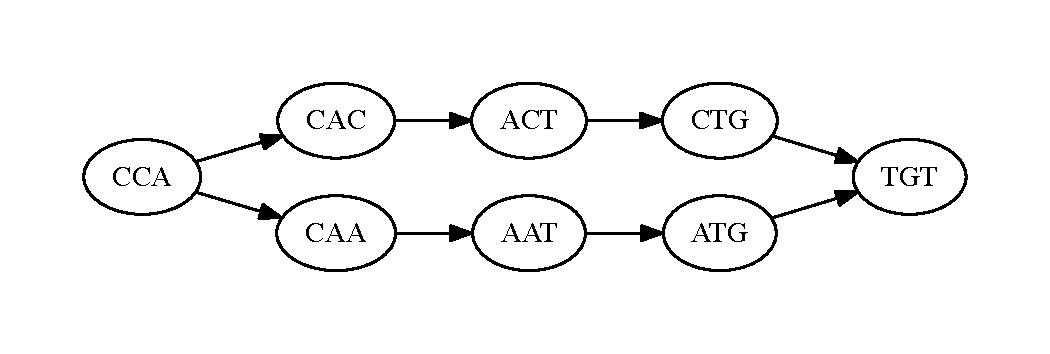
\includegraphics[width=0.95\linewidth, clip=true, trim=0 39 0 39]{graphs/sne.pdf}
\end{center}
\caption{Subgraph Corresponding To a Single Nucleotide Edit}
\label{fig:sne}
\end{figure}

If $m_i = k - 1, m_j \ge k$ or vice versa, we have a canonical INDEL edit (for convenience, we assume
that $\mathcal{S}_i'$ contains the $k - 1$ length path). Here, we can prove that there is a $m_j - m_i$
length insertion in $\mathcal{S}_j'$ relative to $\mathcal{S}_i'$, $k - 1$ letters \emph{after}
$\text{index}(s_1)$:

\begin{lemma}[Distance between $k$ length subsequences]
\label{lem:minimum-distance}
\emph{Indexed de Bruijn} graphs naturally provide a distance metric for $k$ length substrings. Let us construct an
indexed de Bruijn graph $G$ with $k$-mers of length $k$ from a non-repetitive sequence $\mathcal{S}$.
For any two $k$-mers $s_a, s_b \in \mathcal{S}, s_a \ne s_b$, the
$\text{distance}_\mathcal{S}(s_a, s_b)$ metric is equal to $l_p + 1$, where $l_p$ is the length of the
path (in $k$-mers) between $s_a$ and $s_b$. Thus, $k$-mers with overlap of $k - 1$ have an edge
directly between each other ($l_p = 0$) and a distance metric of 1. Conversely, two $k$-mers that are
adjacent but not overlapping in $\mathcal{S}$ have a distance metric of $k$, which implies $l_p = k - 1$.
\end{lemma}

\begin{proof}[Proof regarding Canonical INDELs]
\label{proof:canonical-indels}
We are given a graph $G$ which is constructed from two non-repetitive sequences $\mathcal{S}_i'$ and
$\mathcal{S}_j'$, where the only two $k$-mers in both $\mathcal{S}_i'$ and $\mathcal{S}_j'$ are $s_1$
and $s_2$ and both sequences provide independent paths between $s_1$ and $s_2$. By
Lemma~\ref{lem:minimum-distance}, if the path from $s_1 \rightarrow \dots \rightarrow s_2 \in
\mathcal{S}_i'$ has length $k - 1$, then $\mathcal{S}_i'$ is a string of length $2k$ that is formed by
concatenating $s_1, s_2$. Now, let us suppose that the path from $s_1 \rightarrow \dots \rightarrow s_2
\in \mathcal{S}_j'$ has length $k + l - 1$. The first $l$ $k$-mers after $s_1$ will introduce a $l$ length
subsequence $\mathcal{L} \subset \mathcal{S}_j', \mathcal{L} \not\subset \mathcal{S}_i'$, and then the
remaining $k - 1$ $k$-mers in the path provide a transition from $\mathcal{L}$ to $s_2$. Therefore,
$\mathcal{S}_j'$ has length of $2k + l$, and is constructed by concatenating $s_1, \mathcal{L}, s_2$.
This provides a canonical placement for the inserted sequence $\mathcal{L}$ in $\mathcal{S}_j'$ between
$s_1$ and $s_2$.
\end{proof}

To visualize the graph corresponding to a canonical INDEL, take the two example sequences
\textsc{CACTGT} and \textsc{CACCATGT}. Here, we have a \textsc{CA} insertion after position two. With
$k$-mer length $k = 3$, this corresponds to the graph in Figure~\ref{fig:indel}.

\begin{figure}[h]
\begin{center}
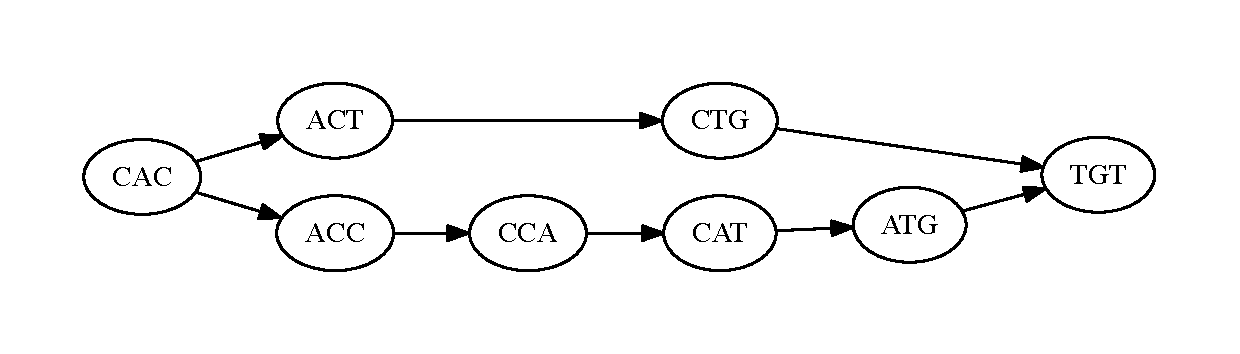
\includegraphics[width=0.95\linewidth, clip=true, trim=0 39 0 39]{graphs/indel.pdf}
\end{center}
\caption{Subgraph Corresponding To a Canonical INDEL Edit}
\label{fig:indel}
\end{figure}

Where we have a canonical allele, the cost of computing the edit is set by the need to walk the graph
linearly from $s_1$ to $s_2$, and is therefore $\mathcal{O}(n)$. However, in practice, we will see
differences that cannot be described as one of the earlier two canonical approaches. First, let us
generalize from the two above proofs: if we have two independent paths between $s_1, s_2$ in the
de Bruijn graph $G$ that was constructed from $\mathcal{S}_i, \mathcal{S}_j$, we can describe
$\mathcal{S}_i$ as a sequence created by concatenating $s_1, \mathcal{L}_i, s_2$. This
property holds true for $\mathcal{S}_j$ as well. The canonical edits merely result from special cases:

\begin{itemize}
\item In a canonical substitution edit, $l_{\mathcal{L}_i} = l_{\mathcal{L}_j} = 1$.
\item In a canonical INDEL edit, $l_{\mathcal{L}_i} = 0, l_{\mathcal{L}_j} \ge 1$.
\end{itemize}

Conceptually, a non-canonical edit occurs when two edits occur within $k$ positions of each other. In
this case, we can trivially fall back on a $O(nm)$ local alignment algorithm~(e.g., a pairwise HMM or
Smith-Waterman, see Durbin et al~\cite{durbin98} or Smith and Waterman~\cite{smith81}), \emph{but} we only need to locally realign
$\mathcal{L}_i$ against $\mathcal{L}_j$, which reduces the size of the realignment problem. However, we
can further limit this bound by limiting the maximum number of INDEL edits to $d = | l_{\mathcal{L}_i} -
l_{\mathcal{L}_j} |$. This allows us to use an alignment algorithm that limits the number of INDEL
edits~(e.g., Ukkonen's algorithm~\cite{ukkonen85}). By this, we can achieve $O(n(d + 1))$ cost.
Alternatively, we can decide to not further canonicalize the site, and to express it as a combined
insertion and deletion. For simplicity and performance, we use this approach in \textsc{Avocado}.

\subsection{Implementation}
\label{sec:implementation}

As alluded to earlier in this section, we can use this indexed de Bruijn concept
to canonicalize INDEL variants without needing to first build a de Bruijn graph.
The insight behind this observation is simple: any section of a read alignment
that is an exact sequence match with length greater than our $k$-mer length maps
to a section of the indexed de Bruijn graph where the read and reference paths
have converged. As such, we can use these segments that are perfect sequence
matches to anchor the bubbles containing variants (areas where the read and
reference paths through the graph diverge) without first building a graph.
We can perform this process simply by parsing the CIGAR string~(and MD tags)
for each read~\cite{li09}. We do this by:

\begin{itemize}
\item Iterating over each operator in the CIGAR string. We coalesce the operators
into a structure that we call an ``alignment block'':
\begin{itemize}
\item If the operator is a sequence match~(CIGAR \textsc{=}, or CIGAR \textsc{M}
with MD tag indicating an exact sequence match) that is longer than our $k$-mer
length, we can create an alignment block that indicates a convergence in the
indexed de Bruijn block~(a sequence match block).
\item If the sequence match operator is adjacent to an operator that indicates
that the read diverges from the reference~(insertion, deletion, or sequence
mismatch), we then take $k$ bases from the start/end of the matching sequence
and append/prepend the $k$ bases to the divergent sequence. We then create an
alignment block that indicates that the read and reference diverge, along with
the two diverging sequences, flanked by $k$ bases of matching sequence on
each side. We call these blocks realignment blocks.
\end{itemize}
\item We then loop over each alignment block. Since the sequence match blocks
are exact sequence matches, they do not need any further processing and can be
directly emitted as a CIGAR \textsc{=} operator. If the block is a realignment
block, we then apply the observations from~\S\ref{sec:formulation}. Again, we
can apply our approaches without building de Bruijn graphs for the bubble.
Specifically, both of the canonical placement rules that we formulate
in~\S\ref{sec:formulation} indicate that the variant in a bubble can be recovered
by trimming any matching flanking sequence. We begin by trimming the matching
sequences from the reference and read, starting from the right, followed
by the left. We then emit a CIGAR insertion, deletion, or sequence
mismatch~(\textsc{X}) operator for this block, along with a match operator if
either side of the flanking sequence was longer than $k$.
\end{itemize}

This process is very efficient, as it can be done wholly with standard string
operators in a single loop over the read. To avoid the cost of looking up the
reference sequence from a reference genome, we require that all reads are
tagged with the SAM \textsc{MD} tag. This allows us to reconstruct the
reference sequence for a bubble from the read sequence and CIGAR.

One problem with this method is that it can be misled by sequencing errors
that are proximal to a true variant. As can be seen in~\S\ref{sec:accuracy},
solely using our indexed de Bruijn algorithm to clean up INDEL alignments leads
to lower accuracy than the state-of-the-art toolkit. However, if the INDEL
variant in a read that is discovered is a true variant, it is a good candidate
to be used as an input to a local realignment scheme.  To implement this
approach, we used our indexed de Bruijn algorithm to canonicalize INDEL variants,
and then we used our variant discovery algorithm~(see~\S\ref{sec:discovery})
with filtration disabled to collect all canonical INDELs. We then fed these
INDELs and our input reads into \textsc{ADAM}'s INDEL realignment
engine~\cite{massie13, nothaft15}. This tool is based on the algorithms used in
the \textsc{GATK}'s INDEL realigner~\cite{depristo11}, and calculates the quality-score
weighted Hamming edit distance between a set of reads, a consensus sequence~(a
haplotype containing a potential INDEL variant), and the reference sequence. If
the sum weighted edit distance between the reads and the consensus sequence
represents a suffient improvement over the sum weighted edit distance between
the reads and the reference genome, the read alignments are moved to their
lowest weighted edit distance position relative to the consensus sequence.
A detailed description of this algorithm can be found in~\S\ref{sec:indel-realignment-implementation}.
As seen in~\S\ref{sec:accuracy}, coupling local realignment with our INDEL
canonicalization scheme improves SNP calling accuracy to comparable with the
state-of-the-art, while improving INDEL calling accuracy by 2--5\%.

\section{Genotyping}
\label{sec:genotyping}

\textsc{Avocado} performs genotyping as a several stage process where variants
are discovered from the input reads and filtered, joined back against the input
reads, and then scored. We use a biallelic likelihood model to score
variants~\cite{li11}, and run all stages in parallel. Our approach does not
rely on the input reads being sorted, and as such, is not unduly impacted by
variations in coverage across the genome. This point is critical in a parallel
approach, as coverage can vary dramatically across the genome~\cite{pinard06}.
If the input reads must be sorted, this can lead to large work imbalances
between nodes in a distributed system, which negatively impacts strong scaling.
An alternative approach is to use previously known data about genome coverage
to statically partition tasks into balanced chunks~\cite{chiang15}. Unlike the
static partitioning approach used by \textsc{SpeedSeq} that discards regions with
very high coverage, this allows us to call variants in regions with very high
coverage. However, as is also noted in the \textsc{SpeedSeq} paper, variant calls
in these regions are likely to be caused by artifacts in the reference genome that
confound mapping and thus are uninformative or spurious, and are hard filtered by
our pipeline~(see~\S\ref{sec:variant-filtration}).

\subsection{Variant Discovery and Overlapping}
\label{sec:discovery}

To identify a set of variants to score, we scan over all of the input reads,
and generate a set of variants per read where each variant is tagged with the
mean quality score of all bases in the read that were in this variant. We then
use \textsc{Apache Spark}'s \textsc{reduceByKey} functionality to compute
the number of times each variant was observed with high quality. We do this
to discard sequence variants that were observed in a read that represent a
sequencing error, and not a true variant. By default, we set the quality
needed to consider a variant observation as high quality to Phred 18~(equivalent
to a error probability of less than 0.016), and we require that a variant is
seen in at least 3 reads. To score the discovered variants, we use the overlap
join primitive introduced in~\S\ref{sec:query-patterns} to find all of the
variants that a single read overlaps. Our implementation uses a broadcast
strategy, as the set of variants to score is typically small and this approach
eliminates the work imbalance problem introduced earlier.

\subsection{Genotyping Model}
\label{sec:genotyping-model}

Once we have joined our reads against our variants, we score each read using
a variant of the biallelic genotyping model proposed by Li~\cite{li11}. Our
approach differs in several ways:

\begin{itemize}
\item Due to the limited numerical precision of double-length floating point
  numbers, we implement our likelihood model entirely in log space. To avoid
  computing logs repeatedly, we tabulate all the possible values of a single
  read's contribution to the likelihood of a single variant given a fixed range
  of base and mapping qualities.
\item To handle multi-allelic sites, we decompose the likelihood model further.
  Specifically, we compute the likelihood that the read supports the reference
  allele, the alternate allele under test, another observed alternate allele,
  or an allele that was not observed. We can use this approach to compute the
  likelihood of a compound heterozygous variant, and to make a partial no-call.
\end{itemize}

An early variant of \textsc{Avocado} used a strict biallelic model, but this
generated incorrect calls for compound heterozygous sites and INDEL variants.
This version of \textsc{Avocado} performed the following process to score variants.
For each variant, we check to see if the read supports the variant allele.
position in the alignment. If the variant is present, we treat the read as positive
evidence supporting the variant. If the read contains the reference allele at
that site, we treat the read as evidence supporting the reference. If the read
neither matches the variant allele nor the reference, we do not use the read
to calculate the genotype likelihoods, but we do use the read to compute
statistics~(e.g., for calculating depth, strand bias, etc.) about the genotyped
site. This version calculated the genotype likelihood for the genotype in log space,
using Equation~\eqref{eq:genotype-likelihood}. Equation~\eqref{eq:genotype-likelihood}
is not our contribution and is reproduced from Li~\cite{li11}, but in log space.

\begin{align}
\label{eq:genotype-likelihood}
\log \mathcal{L}(g) &= -m k \sum_{i = 0}{j} l_r(g, m - g, \epsilon_i) \sum_{i = j + 1}^k l_r(m - g, g, \epsilon_i) \\
l_r(c_r, c_a, \epsilon) &= \text{logsum}(\log c_r + \log \epsilon, \log c_a + \text{logm1}(\log \epsilon))
\end{align}

In Equation~\eqref{eq:genotype-likelihood}, $g$ is the genotype state~(number of
reference alleles), $m$ is the copy number at the site, $k$ is the total number of
reads, $j$ is the number of reads that match the reference genome, and $\epsilon$
is the error probability of a single read base, as given by the harmonic mean of the
read's base quality, and the read's mapping quality, if present. The logsum function
adds two numbers that are in log space, while logm1 computes the additive inverse of
a number in log space. These functions can be implemented efficiently while preserving
numerical stability~\cite{durbin98}. By doing this whole calculation in log space,
we can eliminate issues caused by floating-point underflow. Additionally, since
$\epsilon$ is derived from Phred scaled quantities and is thus already in log
space (base ten), while $g$ and $m - g$ are constants that can be pre-converted to
log space. For all sites, we also compute a reference model that can be used in
joint genotyping in a quasi-gVCF approach. Additionally, we support a gVCF mode where
all sites are scored, even if they are not covered by a putative variant.

The new scoring model used in \textsc{Avocado} checks to see if the read matches
the alternate allele we are testing, the reference allele, another alternate
allele that overlaps with the allele we are testing, or none of the above. 
To do this, we use the ``one sided'' variant of
Equation~\eqref{eq:genotype-likelihood}, which is given in
Equation~\eqref{eq:one-sided}.

\begin{align}
\label{eq:one-sided}
\log \mathcal{L}(g) &= \sum_{i = 0}{j} l_r(g, m - g, \epsilon_i)
\end{align}

For all sites, the log sum of the one-sided likelihood of the reference allele
and the one-sided likelihood of the alternate allele under test will be equal to
the value of the full biallelic likelihood model. However, the one-sided model
can also be applied to sites with more than one alternate allele. For these
sites, after computing all one-sided likelihoods, we then calculate the combined
likelihoods for each pair of alleles, and emit a genotype call that corresponds
to the highest likelihood of all admissible likelihood combinations.

We compute the likelihoods for each read in parallel. The scoring function maps
over all of the reads. For each variant covered by the read being observed, the
scoring function will emit a record that contains the mapping and base
qualities, and whether the read supported the reference allele, the alternate
allele under test, another alternate allele, or no known alleles. These records
are converted into a \textsc{Spark SQL} DataFrame, and we join these values
against a small table containing all of the pre-computed one-sided likelihoods.
We then run an aggregation over all reads covering a given variant, for all
variants in parallel. Once we have aggregated all of the observations for a given
site, we call the genotype state by taking the genotype state with the highest
likelihood. In single sample mode, we assume no prior probability.

\subsection{Variant Filtration}
\label{sec:variant-filtration}

Once we have called variants, we pass the calls through a hard filtering engine.
First, unless we are in gVCF mode, we discard all homozygous reference calls and
low quality genotype calls (default threshold is Phred 30). Additionally, we
provide several hard filters that retain the genotype call, but mark the call as
filtered. These include:

\begin{enumerate}
\item Quality by depth: the Phred scaled genotype quality divided by the depth at
the site. Default value is 2.0 for heterozygous variants, 1.0 for homozygous
variants. The value can be set separately for INDELs and SNPs.
\item Root-mean-square mapping quality: Default value is 30.0 for SNPs. By default,
this filter is disabled for INDELs.
\item Depth: We filter out genotype calls below a minimum depth, or above a maximum
depth. By default, the minimum depth is 10, and maximum depth is 200. This value
can be set separately for INDELs and SNPs.
\end{enumerate}

\part{Evaluation}

\chapter{Benchmarking the \textsc{ADAM} Stack}
\label{chap:benchmarking}

\section{Benchmarking Preprocessing Algorithms}
\label{sec:benchmarking-preprocessing}

\subsection{Benchmarking Duplicate Markers}
\label{sec:benchmarking-duplicate-markers}

\subsection{Benchmarking INDEL Realigners}
\label{sec:benchmarking-indel-realigners}

\subsection{Benchmarking Recalibrators}
\label{sec:benchmarking-recalibrators}

\section{Evaluating Compression Techniques}
\label{sec:compression}

These representations achieve high compression versus the legacy formats. We provide a detailed breakdown of
compression in~\S\ref{sec:compression}. \textsc{ADAM} data stored in \textsc{Parquet} achieves an
approximately 25\% reduction in file size over compressed \textsc{BAM} for read data, and a 66\% reduction
over \textsc{GZIP}ped \textsc{VCF} for variant data.

\section{Benchmarking \textsc{Cannoli}}
\label{sec:benchmarking-cannoli}

\chapter{The Simons Genome Diversity Dataset Recompute}
\label{chap:sgdd}

\part{Conclusion and Future Work}

\chapter{Future Work}
\label{chap:future-work}

\begin{itemize}
\item What were our overarching the goals?
  \begin{itemize}
  \item Make genomic analysis easier to scale
  \item Improve variant calling accuracy
  \item Make genomic data analysis faster
  \end{itemize}
\item Several future directions:
  \begin{itemize}
  \item Further improving query performance in \textsc{ADAM}
  \item Extending variant calling algorithms in \textsc{Avocado}
  \item Hardware acceleration for genomics
  \end{itemize}
\end{itemize}

\section{Further Query Optimization in \textsc{ADAM}}
\label{sec:extensions-adam}

\begin{itemize}
\item Preserving sorted knowledge in \textsc{ADAM}
  \begin{itemize}
  \item Needed to improve performance of region joins
  \item Currently implemented, but refactoring to extend to legacy genomic datatypes
  \item Store sorted state as metadata in the GenomicRDD.
  \end{itemize}
\item Extending what transformations can be optimized by partitioning:
  \begin{itemize}
  \item Currently just accelerate joins
  \item Aggregation queries naturally fall out of this as well
  \end{itemize}
\item Exposing other primitives as well:
  \begin{itemize}
  \item Convex hull merge
  \end{itemize}
\end{itemize}

\section{Extensions to \textsc{Avocado}}
\label{sec:extending-avocado}

\begin{itemize}
\item Deep learning for variant calling:
  \begin{itemize}
  \item Current model for INDEL discovery is intolerant of read errors
  \item Doesn't model error distribution over technologies
  \item Google \textsc{DeepVariant} uses deep learning but in an unglamorous way
  \item Would the \textsc{Avocado} INDEL canonicalization algorithm be a better fit?
  \end{itemize}
\item Somatic variant calling:
  \begin{itemize}
  \item \textsc{Avocado} currently only models a sample with known ploidy
  \item Can we accomodiate pooled or somatic variant calling?
  \item WIP towards porting over MuTect
  \end{itemize}
\end{itemize}

\section{Hardware Acceleration for Genomic Data Processing}
\label{sec:genomic-hardware}

\begin{itemize}
\item With improved I/O, single thread performance remains an issue
  \begin{itemize}
  \item As seen with \textsc{Cannoli}, hard to outperform C++ from Java
  \item However, marginal benefit to jumping to C++ is unclear
  \item Can we go directly to hardware?
  \end{itemize}
\item WIP on Genie library
\item How can we make this even more accessible?
  \begin{itemize}
  \item SQL as target language is a great opportunity
  \item Integrate Genie with Apache Arrow
  \item Allow generation of FPGA from Spark SQL plan
  \end{itemize}
\item How can we easily accomodate UDFs?
\end{itemize}

\section{Improved Metadata Management for Genomics}
\label{sec:metadata-future}

\section{Efficient Consensus Methods}
\label{sec:efficient-consensus}

\section{Improving Debugging Capabilities for Distributed Systems}
\label{sec:improving-debug}

\section{Lazily Binding To Genomic File Formats}
\label{sec:lazy-bind}

\chapter{Conclusion}
\label{chap:conclusion}

\backmatter

\bibliographystyle{abbrv}
\bibliography{fnothaft-phd-thesis}

\end{document}
